% arara: pdflatex
% arara: nomencl
% arara: pdflatex
\documentclass[a4paper,11pt]{mscThesis}

%
%========================== Packages ======================================
		\usepackage{lipsum} 
		\usepackage{outlines}
		\usepackage{amsmath}
		\usepackage{amssymb}
		\usepackage{tabularx}
		\usepackage{graphicx}
		\usepackage{subfig}
		\usepackage{hhline}
		\usepackage{epstopdf}
		\usepackage{url}
		\usepackage{enumitem}			
		
		\usepackage[framed,numbered,autolinebreaks,useliterate]{mcode}
		
		% Acronyms
		\usepackage{acronym}
		%Nomenclature
		\usepackage{nomencl}
		\makenomenclature		
		%Index package
		\usepackage{imakeidx}		
		\makeindex
		
		\renewcommand{\a}[1]{\acs{#1}} %Fastkey \acs{[1]}
		\renewcommand{\v}[1]{\vspace{-#1mm}} 
		\newcommand{\IF}{$\left\lbrace\mathcal{I}\right\rbrace$ }
		\newcommand{\BF}{$\left\lbrace\mathcal{B}\right\rbrace$ }	
		\newcommand{\dir}[1]{C:/Users/Nam/Documents/Git/Thesis-Quadrotor-Code/NamMatlab/QRL/MatlabImages/{#1}.png}
		
		\setcounter{MaxMatrixCols}{20}
	
		%Tabitems
		\usepackage{booktabs}% http://ctan.org/pkg/booktabs
		\newcommand{\tabitem}{~~\llap{\textbullet}~~}
		
		% Bibliography
		\usepackage[utf8]{inputenc}

%================================================================		

\mscDepartment{Delft Center for Systems and Control}
%{Systems and Control}
\mscProgram{Mechanical Engineering} \mscFaculty{Mechanical,
Maritime and Materials Engineering} \mscName{N.N. Vo}
\mscDate{\today} \mscTitle{Geometric Control of a Quadrotor with a Suspended Load} \mscSubTitle{Subtitle}
\mscKeyWords{thesis, msc, subject}
%
%use the next line if you want a picture on the title page
\mscTitlePagePicture{example_titlefig}
%Note: the file example_titlefig.eps is just for illustration. Do not use this for your own thesis

%% --------------------------------------------------------------------
%% THIRD PARTY OPTIONS

%use the next line if you want a text to acknowledge (a) third party/parties on the copyright page
\mscThirdPartyText{The work in Master of Science Thesis was supported by Alten. Their cooperation is hereby gratefully acknowledged.}

%use the next line if you want the logo of a third party on the copyright page
%NOTE: on the title page only the TUDelft and DCSC logo's are permitted. These are automatically created

\mscThirdPartyLogo{./StyleStuff/ALTEN.png}
%Note: the file examplelogo.eps is just for illustration. Do not use this for your own thesis

%% --------------------------------------------------------------------


\mscReaderOne{dr.ir. T. Keviczky}
\mscReaderTwo{ir. B. van Vliet}
%\mscReaderThree{ir. My. Readertwo}
%\mscReaderFour{}
%
\setThesisInfo
%

\begin{document}
%
%============================= Front matter ========================================
\frontmatter %
%
% Make a hell of a lot of title pages
 \maketitle
%
% Abstract
\nonumchap{Abstract}
\vspace{-2cm}
A quadrotor is a type of Unmanned Aerial Vehicle that has received an increasing amount of attention recently with many applications being actively investigated. 
Possible applications include search and rescue, surveillance, supply of food and medicines in emergency situations and object manipulation in construction and transportation.
An interesting subproblem of load transportation is the control of the position of a cable suspended load. The challenge is in the fact that the quadrotor-load system is highly nonlinear and under-actuated. The load cannot be controlled directly and has a natural swing at the end of each quadrotor movement. 

The goal of this thesis is to present a nonlinear geometric control approach, investigate its possibilities and limitations to track the position of a cable suspended load. The focus lies on the quadrotor-load subsystem where the cable tension is non-zero, which is analogous to modeling a rigid link between the quadrotor and load.
%The main goal is to investigate the possibilities and limitations of nonlinear geometric control for the purpose of load trajectory tracking of a quadrotor with a cable-suspended load, by evaluating the stability of the system and the tracking performance on different load trajectories. 

After introducing the basic concepts, an introduction is given on geometric mechanics. This differential geometric based approach is used model and control the system, based on the geometric properties of the system dynamics. 
It is shown how the configuration of the quadrotor-load system can be described on smooth nonlinear geometric configuration spaces, and analyzed with the principles of differential geometry. 
This allows for modeling in an unambiguous coordinate-free dynamic fashion, while avoiding the problem of singularities that would occur on local charts. \\
%Next, the quadrotor-load system is modeled with the tools of differential geometry in order 
%to make it suitable for nonlinear geometric control. T
Next, the geometric properties are utilized to define tracking error functions on these same spaces, making it possible to design almost-globally defined nonlinear geometric controllers. A backstepping approach is applied to generate a cascaded structure with multiple nonlinear geometric controllers, allowing control of several flight modes that are responsible for the control of 1) quadrotor attitude, 2) load attitude and 3) load position.\\ 
Finally, simulations demonstrate the stability and abilities of the nonlinear geometric controller. A Linear Quadratic Regulator is derived to compare control performance. The tracking performances of both controllers are discussed for three different experiments and final conclusions are presented. The thesis is concluded with a summary and recommendations for future work.
 

%%CHANGE meer power / eye cather, wat gebeurt er in deze thesis
%Different cases are tested to investigate the possibilities and limitations of nonlinear geometric control. 
%%ADD Results show
%Results show that....
%
%
%***************************************\\
%Intro about GC.. 
%Reasons to consider GC..
%
%***************************************\\
%Where simple linear control methods are restricted to small angle movements, nonlinear control methods allow more aggressive and faster movements.  The goal of the project is to investigate the effects on load position tracking performance when the system is modeled and controlled via a nonlinear geometric control approach.
%
%
%***************************************\\
%The quadrotor-load system is modeled in a compact and coordinate-free fashion which allows the inherent geometric properties of the system to be controlled. 
%%BOVENSTAAND IS VAAG?

%
%The main goal of this thesis is to research the effects on a cable-suspended load transportation using quadrotors, by involving complex or aggressive maneuvering through implementation of Non-Linear geometric control.
%Where linear control methods are restricted to small angle movement, non-linear control methods allow more aggressive movements. 

%
%		The main goal of this literature study is to review researches that have been done regarding the possibilities of manipulation and transportation of cable-suspended loads using quadrotors, possibly involving complex or aggressive maneuvering. Where linear control methods are restricted to small angle movement, non-linear control methods allow more aggressive movements, but are subject to complex 
%		***************************************\\
%		What is complex? If that results in super easy feedback loop, why not consider it?
%		
%		***************************************\\
%		mathematics and are more computationally intensive and less robust. 


%***************************************\\
%In the considered research papers, different modeling methods and control techniques are applied which are suitable for various specific applications. The models, derivation and underlying assumptions are studied and explained in detail. 		
%
%Super general. Can be placed in every paper.
%
%***************************************\\

%Furthermore, the studied control techniques are explained and their advantages are addressed. Several trajectory generation approaches and the related optimization techniques are studied. Their applications, with different purposes such as obstacle avoidance, time-optimal and swing-free trajectory planning are explained. The survey is concluded with a discussion about finding a suitable
%***************************************\\
%Define suitable
%
%***************************************\\
%control design to achieve the quadrotor-assisted task involving manipulation of a cable-suspended load.
%
%***************************************\\


		
\cleardoublepage
%
% Acknowledgements
    \nonumchap{Acknowledgements}%
    I would like to thank my supervisors \mscreaderone\ from Delft Center of Systems and Control, and \mscreadertwo\ from Alten Nederland B.V. for their assistance during my research and the writing of this thesis. I would also like to thank all colleagues from Alten and TU Delft for their time and advices.
    \vspace*{15mm}

    \noindent
    Delft, University of Technology \hfill \mscname\\
    \mscdate

%
% table of contents, (\toc of \toclof of \tocloflot )
    \tocloflot
%
    
    \cleardoublepage%
%
%============================= Main matter =========================================
%
\mainmatter
%
% Introduction
%\include{examples}
%FROM LITERATURE
%\chapter*{Plan of approach}

Geometric Control looks most promising for attitude tracking of the QR and includes the ability to maneuver aggressively. To build almost-globally attractive controllers, stability of the error dynamics must be proven in order to guarantee the overall stability of the complete dynamics. Based on Geometric Control, Hybrid Control considers the different dynamics of a quadrotor-load system and makes this is a potential candidate for the position tracking of the load and attitude tracking of the quadrotor.

Minimizing Snap Trajectory Generation, where a Quadratic Programming problem is solved, looks most promising in terms of computational load and feasibility to generate an aggressive, yet smooth trajectory for both quadrotor and quadrotor-load systems. Obstacle avoidance constraints can be added by using integer variables and solving a Mixed Integer Quadratic Programming problem.

The goal is to make a control design for the QR-Load system based on Geometric Modeling and Geometric Control, which is capable of tracking a load trajectory, while maintaining the attitude control of the QR. The objective is divided into subproblems and the following approach is proposed to achieve this objective.

The feasibility of the nonlinear geometric control design has to be shown for the QR system, before involving the dynamics of a suspended load. Next, it must be proven that the proposed Hybrid Control of the QR-Load system is able to track a load trajectory, allowing switches between the QR-Load subsystem and QR subsystem. By defining a trigonometric function, the trajectory tracking can be tested in a controlled manner. A trajectory can be optimized by minimizing an objective function of the fourth and sixth derivative of position w.r.t. time, which is able to take various constraints into account by using the properties of differential flatness.
\section{QR System}
\begin{outline}
\1 Modeling QR system, using geometric algebra and Lie algebra
\begin{align}
	\dot{x}&=v\\
	m\dot{v}&=mge_3-fRe_3\\
	\dot{R}&=R\hat{\Omega}\\
	M&=J\dot{\Omega}+\Omega\times J\Omega
\end{align} 
\1 Simulation using:
\2 Simulink
\2 MATLAB
\2 MATLAB Robotics Toolbox \footnote{\url{http://www.petercorke.com/RTB/robot.pdf}}												
\1 Reproduce Geometric Position Control							
\1 Reproduce Geometric Attitude Control	
\1 Reproduce Trajectory Generation
\1 Incorporate effects of model- and parameter uncertainties
\begin{align}
\dot{x}&=v\\
m\dot{v}&=mge_3-fRe_3+\Delta_x\\
\dot{R}&=R\hat{\Omega}\\
M+\Delta_R&=J\dot{\Omega}+\Omega\times J\Omega
\end{align} 
where $ \Delta_x $ and $ \Delta_R \in\mathbb{R}^3$ denote unstructured, but fixed uncertainties in the translational and rotational dynamics.
\1 Incorporate effects of sensor noise and filters							
\1 Simulation including effects of implementation
\end{outline}						

If the feasibility of the nonlinear geometric control design is shown, the QR-Load system is considered by incorporating the dynamic effects of the load. 
For the QR-Load system, the same approach as in the previous section is used. Simulation must prove the feasibility of the theories.
\section{QR-Load System}
\begin{outline}
	\1 Modeling of the QR-Load system, using geometric algebra and Lie algebra.
	For the QR-Load Subsystem, with non-zero cable tension
	\begin{align}
	\dot{x}_L&=v_L\\
	(m+m_L)(\dot{v}_L+ge_3)&=(q\cdot fRe_3-ml(\dot{q}\cdot\dot{q}))q\\
	\dot{q}&=\omega\times q\\
	ml\dot{\omega}&=-q\times fRe_3\\
	\dot{R}&=R\hat{\Omega}\\
	M&=J\dot{\Omega}+\Omega\times J\Omega
	\end{align} 

	For the QR Subsystem, with zero cable tension
	\begin{align}
	\dot{x}_L&=v_L\\
	m_L(\dot{v}_L+ge_3)&=0\\
	\dot{x}&=v\\
	m\dot{v}&=mge_3-fRe_3\\
	\dot{R}&=R\hat{\Omega}\\
	M&=J\dot{\Omega}+\Omega\times J\Omega
	\end{align} 
	
	\1 Hybrid Control Design	
	\begin{align}
	\Sigma_n&=\begin{cases}
	\dot{X}_n=f_n(X_n)+g_n(X_n)u, & X_n\notin\mathcal{S}_z\\
	X^+_z=\Delta_{n\rightarrow z}(X_n^-), & X_n\in\mathcal{S}_z
	\end{cases}\\	
	\Sigma_z&=\begin{cases}
	\dot{X}_z=f_z(X_z)+g_z(X_z)u, & 	X_z\notin\mathcal{S}_n\\
	X_n^+=\Delta_{z\rightarrow n}(X_z^-),& 	X_z\in\mathcal{S}_n
	\end{cases}	
	\end{align}
	where
	\begin{align}
	X_n&=\left\{x_L,q,R,v_L,\omega,\Omega\right\}\\
	X_z&=\left\{x_L,x_Q,R,v_L,v_Q,\Omega\right\}\\
	u&=\left\{f,M\right\}\\
	&\text{Where the guards are defined as}\\
	\mathcal{S}_n&=\left\{X_z|\parallel x_Q-x_L\parallel\equiv l,\frac{d}{dt}\parallel x_Q-x_L\parallel>0\right\}\\
	\mathcal{S}_z&=\left\{X_n|T\equiv0\right\}\\
	&\text{Where the tension is defined as}\\
	T&:=\parallel m_L(\ddot{x}_L+ge_3)\parallel
	\end{align}
	where $ \Delta_{n\rightarrow z} $ is an identity map, and $ \Delta_{z\rightarrow n} $ is modeled as an inelastic collision of two objects, that ensures $ \dot{x}_Q^+-\dot{x}_L^+=0 $.

	\2 Test for the planar 2-D case 
	\2 Test for the full 3-D case	
	\3 Reproduce Geometric Attitude Control	for QR	
	\3 Reproduce Geometric Attitude Control	for Load	
	\3 Reproduce Geometric Position Control	for Load						
	\3 Reproduce Trajectory Generation for Load
		
\section{Trajectory Generation}
Minimizing the sixth-derivative of the load position ensures minimum snap motion for the QR. The following must be solved,
\begin{equation}\label{key}
\min \int_{t_0}^{t_1}\parallel\frac{d^kx_i}{dt^k}\parallel^2dt
\end{equation}
\1 \textbf{Obstacle avoidance}
\2 Trajectory generation, as done by \cite{Tang2015}
\end{outline}				


\section{QR System Implementation}		
\begin{outline}
\1 Set up communication with Optitrack, Paparazzi's Nat2Ivy
\1 Set up manual control and use known \a{uav} parameters for modeling
\1 Test Geometric Position Control with existing Attitude Control 
\1 Test Geometric Attitude Control				

\1 \textbf{Optional; Improve Model}
\2 System identification with \textbf{\a{indi}}\cite{Smeur2015,Smeur2016}
\2 Evaluate the validity of identified system
\2 Dynamic modeling of QR system				

\1 \textbf{Optional; Off-board Control }\\
This will allow off-board communication and calculations				
\2 Set up former framework as done by \cite{PraveenThesis}
\end{outline}

%
% Introduction
\chapter{Introduction} \label{chap::intro}

This is a \LaTeX\ thesis and this is Chapter\ \ref{chap::intro}.

\section{About \texorpdfstring{\LaTeX}{LaTeX}}

\LaTeX\ is a document preparation system for the \TeX\ typesetting program. It offers programmable desktop publishing features and extensive facilities for automating most aspects of typesetting and desktop publishing, including numbering and cross-referencing, tables and figures, page layout, bibliographies, and much more.

\LaTeX\ was originally written in 1984 by Leslie Lamport and has become the dominant method for using \TeX; few people write in plain \TeX\ anymore. The current version is \LaTeXe.

If you want to know more about \LaTeX\ you better read \cite{texbook}.\index{LaTeX}


\section{About Acronyms}

This section contains an acronym of the \ac{DCSC}. The \ac{DCSC} is our department within the faculty of \ac{3mE} at \ac{TU}. \index{acronym}

Acronyms are automatically listed in the Glossary in the back of this thesis. You have to define acronyms in \texttt{glossary.tex} using \verb"\acro{ACRONYM}{Full text}". You print an acronym by using the command \verb"\ac{...}". You can always force a full, long or short printout by using \verb"\acf{...}", \verb"\acl{...}" or \verb"\acs{...}" respectively.

\begin{itemize}
    \item \verb"\acf{DCSC}": \acf{DCSC};
    \item \verb"\acl{DCSC}": \acl{DCSC};
    \item \verb"\acs{DCSC}": \acs{DCSC}.
\end{itemize}

\section{About the Nomenclature}

When you use symbols in your thesis -- as you probably will -- you can put them into the nomenclature listing (List of Symbols) at the back of your thesis. \tabref{tab:nomencl} shows the \LaTeX\ commands you need.\index{nomenclature}

\begin{table}%
    \centering
    \caption{Nomenclature codes}
    \label{tab:nomencl}
    \begin{tabular}{llcl}
        \toprule
        Code & Usage & Example\\
        \midrule
        \verb"\gsymb{}" & Greek symbols & \gsymb{$\gamma$}{Path Angle}\\
        \verb"\lsymb{}" & Letter symbols & \lsymb{$H(s)$}{Transfer function}\\
        \verb"\supers{}" & Superscript symbols & \supers{max}{Maximum} &\emph{only printed in the List of Symbols} \\
        \verb"\subs{}" & Subscript symbols & \subs{min}{Minimum} &\emph{only printed in the List of Symbols}\\
        \verb"\others{}" & Other symbols & \others{[kts]}{Knots} \others{$^{\circ}$, [deg]}{Degrees} &\emph{only printed in the List of Symbols}\\
        \bottomrule
    \end{tabular}
\end{table}

\section{About {\textbackslash}(re)newcommand}
As you will (soon) know the \LaTeX\ system makes use of commands in
the form of \verb"\command". This can be used to make your life
easier, since you can also define these commands yourself. Suppose
that you often use an expression $e^{it}$. This would
normally be written as \verb"$e^{it}$", or if already in math mode
as \verb"e^{it}". Now you can define a command
\verb"\eit" as follows\\
\verb"\newcommand{\eit}{e^{it}}"\\
This definition has to be placed in the so-called preamble, i.e.
before the declaration\\ \verb"\begin{document}".\\ Now you can use
this
command in your text, so \verb"\eit" replaces \verb"e^{it}".\\
Be aware that many commands are already in use by various packages.
If you define an already existing command this will result in an
error message. The best way to deal with this is to make sure your
own command is unique, for instance by defining it as\\
\verb"\newcommand{\MYeit}{e^{it}}".\\
An alternative is to redefine the existing command by\\
\verb"\renewcommand{\eit}{e^{it}}",\\
but this is in general considered a tedious practice and should be
avoided.
See the \LaTeX\ documentation for more details and possibilities. You can also use arguments.\\
%
Don't underestimate the power of this feature. Suppose that you
frequently use the expectation operator $E(x)$ in your text which is
created with \verb"E(x)" (in math mode). Now your supervisor decides
that he would prefer to see this as $\bf{E}(x)$. If you haven't
defined your own command, you will have to go through the complete
text, changing every instance. If you would have thought about it
and
would have defined originally\\
\verb"\newcommand{\MyE{1}}{E(#1)}",\\
using this in your text as
\verb"\MyE{x}", \verb"\MyE{y}" etc.,\\
then you can change this simply by adapting the definition to\\
\verb"\newcommand{\MyE{1}}{\bf{E}(#1)}".

\chapter{Dynamic Model} \label{ch:model}

***************************************\\
%INTRO 

The dynamics of the QR-Load system are described by the laws of kinematics and the application of Newton's laws or Lagrangian mechanics. Opposed to the classical modeling techniques, it is also possible to describe the system's configuration space as a differentiable manifold with the tools of differential geometry. \\

In order to simulate the system and the effects of Geometric Control, the system is modeled with the following assumptions.\\

In order to avoid complexities and ambiguities associated with attitude representations such as \textit{Euler-Angles} or \textit{quaternions}, the attitude dynamics of the Quadrotor-Load system can be globally expressed on the Special Orthogonal Group $SO(3)$
***************************************\\

The derived mathematical model is represented by a set of dynamic equations commonly used for rigid body transformations. Considering the properties of the system, the QR is modeled as a rigid body. The motion of a rigid body can be described by a translation of the center of mass and a rotation about the center of mass. This principle describes a rigid body with six degrees of freedom, driven by forces and moments. \\

\section{Modeling Assumptions} 
The Quadrotor model representation is shown in Figure \ref{fig:mod.model}. Three Cartesian coordinate frames are defined:\v{5}
\begin{itemize}
	\setlength\itemsep{.2pt}
	\item The body-fixed reference frame \lsymb{$ \{\mathcal{B}\} $}{Body Frame} (Body Frame)
	%								\nomenclature{$ \{\mathcal{B}\} $}{Body Frame}
	\subitem with unit vectors \lsymb{$ \{\mathbf{b}_1,\mathbf{b}_2,\mathbf{b}_3\} $}{Unit vectors along the axes of $ \{\mathcal{B}\} $} along the axes
	\item The ground-fixed reference frame \lsymb{$ \{\mathcal{I} \}$}{Inertial World Frame} (Inertial Frame)
	%								\nomenclature{$ \{\mathcal{I} \}$}{Inertial World Frame}
	\subitem with unit vectors \lsymb{$ \{\mathbf{e}_1,\mathbf{e}_2,\mathbf{e}_3\} $}{Unit vectors along the axes of $ \{\mathcal{I}\} $} along the axes								
	\item The intermediary frame \lsymb{$ \{\mathcal{C} \}$}{Intermediary Frame}, ($ \{\mathcal{I} \}$ rotated by the yaw angle $ \psi $) 
	%								\nomenclature{$ \{\mathcal{C} \}$}{Intermediary Frame}
	\subitem with unit vectors \lsymb{$ \{\mathbf{c}_1,\mathbf{c}_2,\mathbf{c}_3\} $}{Unit vectors along the axes of $ \{\mathcal{C}\} $} along the axes								
\end{itemize}

\begin{figure}[h!]
	\centering
	\makebox[\textwidth][c]{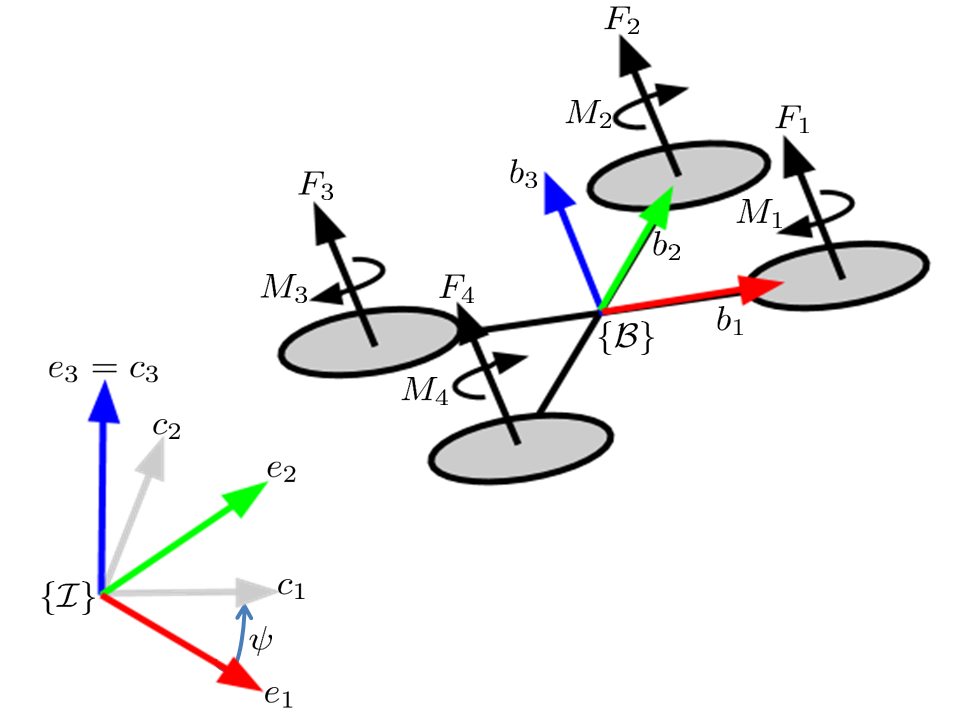
\includegraphics[width=.5\paperwidth]{./StyleStuff/qrmodelppt.png}}
	\caption{Quadrotor model representation\label{fig:mod.model}}
\end{figure}	

\begin{figure}[h!]
	\centering
	\makebox[\textwidth][c]{\includegraphics[width=.5\paperwidth]{./StyleStuff/dcsc.png}}
	\caption{Quadrotor with Load model representation\label{fig:mod.modelQRL}}
\end{figure}	

The position of the body frame is described by a vector evolving on $ \mathbb{R}^3 $, and is represented with respect to the inertial frame. The orientation of the body frame with respect to the inertial frame evolves on a nonlinear space, for which several methods exist to describe this, such as \textit{Euler Angles}, quaternions or rotation matrices. 

Table \ref{tab:mod.assumptions} shows the most common assumptions that are used for modeling the QR, simplifying the complexity of the model.

\begin{table}[h!]
	\centering
	\begin{tabular}{|p{\textwidth}|}
		\hline
		\tabitem The rotation of the Earth does not affect the flight of the QR\\
		\tabitem The structure of the QR is rigid and symmetric. \\
		\hspace{4mm} Elastic deformations and shock (sudden accelerations) of the QR are ignored.\\										
		\tabitem The mass distribution of the QR is symmetrical in the x-y plane.\\
		\tabitem The inertia matrix is time-invariant.\\
		\tabitem Aerodynamic effects acting on the QR are neglected.\\
%		\hspace{4mm} An indoor environment guarantees the absence of unpredictable disturbances like wind\\ 
%		\hspace{4mm} gusts. The model complexity decreases without modeling the effects of wind.\\ 	
		\tabitem The propellers are rigid $ \Rightarrow $ The thrust produced by rotor $ i $ is parallel to the axis of rotor $ i $.\\
		\tabitem The air density around the QR is constant.\\
		\tabitem Drag factor \lsymb{$ d $ }{Drag factor} and thrust factor \lsymb{$ b $}{Thrust factor} are constant.\\
		\hspace{4mm} Thrust force $ F_i $ and drag moment \lsymb{$ \tau_{drag,i} $}{Drag moment generated by each propellor} of each propeller is proportional to the square of \\
		\hspace{4mm} the propeller speed. $ F_i = b\omega_i^2$ and $ \tau_{drag,i} = d\omega_i^2$, where \lsymb{$ \omega_i $}{Angular velocity of rotor $ i $ around its axis, $ i=\{1,2,3,4\} $} is the rotor speed.\\
		\hline
	\end{tabular}
	\caption{Modeling assumptions Quadrotor model}
	\label{tab:mod.assumptions}
\end{table}

\begin{table}[h!]
	\centering
	\begin{tabular}{|p{\textwidth}|}
		\hline
		\tabitem The cable is modeled as a rigid and massless cable. \\
		\tabitem The tension in the cable is considered to be non-zero.\\
		\hspace{4mm} This implies that the subsystem consisting of a Quadrotor and Load in free fall is disregarded.\\		 
		\tabitem Aerodynamic effects acting on the load are neglected.\\
		\tabitem The cable is connected to a friction-less joint at the origin of the body-fixed reference frame.\\
		\tabitem Assumption \\
		\hspace{4mm} Details Assumption 2\\
		\hline
	\end{tabular}
	\caption{Modeling assumptions Quadrotor+Load model}
	\label{tab:mod.assumptionsQRL}
\end{table}



***************************************\\
\cite{Goodarzi2013a} includes uncertainties in the translational dynamics and rotational dynamics. Out of the scope, might be interesting.\\
***************************************\\


***************************************\\
\begin{figure}[h!]
	\centering
	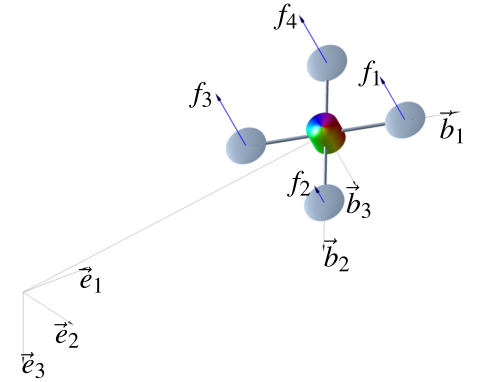
\includegraphics[width=.45\textwidth]{./StyleStuff/LeeQRmodel.png}
	\caption{\label{fig:}}
\end{figure}		
***************************************\\


\section{Geometric Modeling}\label{sec:mod.geometric}

%HOE DAN? 
Differential Geometry is used to analyze the underlying geometric properties of a system.

With geometric modeling the configuration space is a group manifold instead of a Euclidean space. The kinetic and potential energies are expressed in terms of this configuration space and its velocities.

***************************************\\
Rigid Body Attitude Dynamics:
\begin{align}\label{eq:eomrigidbody}
J\dot{\Omega}+\Omega\times J\Omega &= mg\rho\times R^Te_3+u\\
\dot{R} &= R\hat{\Omega}
\end{align}
***************************************\\


***************************************\\
\cite{Lee}
Why is this used, pros/cons\\

%		\subsection{Lagrangian System}
Mechanics studies the dynamics of physical bodies acting under forces and potential fields. 
In Lagrangian mechanics, the trajectories are obtained by finding the paths that minimize the integral of a Lagrangian over time, called the action integral. 
Rigid body dynamics are characterized by Lagrangian/Hamiltonian dynamics. The dynamics of a Lagrangian system has unique geometric properties and these are exploited to obtain Euler-Lagrange equations. The resulting intrinsic form of the Euler-Lagrange equations are more compact than equations expressed in terms of local coordinates.

When angular errors are large, the difference in Euler angles is no longer a good metric to define the orientation error. Local coordinates often require symbolic computational tools due to complexity of multi-body systems. Hence, the error is rather written as the required 3-D rotation to get from the current to the desired orientation. As a result, the equations of motion and the control systems can be developed on a configuration manifold in a coordinate-free, compact, unambiguous manner, while singularities of local parameterization are avoided to generate agile maneuvers in a uniform way. 				

Most of nonlinear dynamics and control problems are studied in a linear space.\\
\begin{equation}\label{key}
\dot{x}=f(t,x,u), \quad x\in\mathbb{R}^n, u\in\mathbb{R}^m, f:\mathbb{R}^{n+m+1}\rightarrow\mathbb{R}^n
\end{equation}

Geometric Mechanics and Control is used to understand the structure of the equations of motion of a system in order to facilitate its analysis and design. The evolution of the system and the design of controllers is done on a nonlinear manifold.\\

In mathematics there are different types of singularity, in these cases we are talking about the situation where:\\
Many points in one representation are mapped onto a single point in another representation.\\
Infinitesimal changes close to the singularity in one representation may cause large changes in the other representation.

Computational Geometric Mechanics and Control\\
Computation algorithms must be developed which preserve the geometric properties of a mechanical system.\\
Robust and careful numerical implementation of geometric control theory to complex engineering systems.\\
Provides nontrivial maneuvers that are globally valid on a nonlinear configuration manifold.

Assumptions\\

Problems, singularities with Euler-Angles\\
Other attitude representations, such as exponential coordinates, quaternions, or Euler
angles, can also be used following standard descriptions, but each of the representations has a disadvantage
of introducing an ambiguity or singularity.
Why charts on $ SO(3) $ \url{https://en.wikipedia.org/wiki/Charts_on_SO(3)}\\

\begin{equation}\label{key}
SO(3) \triangleq \left\lbrace R\in\mathbb{R}^{3\times3}:RR^T=I_{3\times3},det(R)=1\right\rbrace 
\end{equation}

Rotational matrices with determinant 1 is a Lie group: $ SO(3) $\\
$ SO(3) $ is the group of all rotations about origin of three-dimensional Euclidean space\\
Rotation about the origin is a transformation that preserves the origin, Euclidean distance and orientation.\\
Every rotation has a unique inverse rotation and the identity map satisfies the definition of a rotation.\\
Possible ways to represent rotations: orthogonal matrices with determinant 1, axis and rotation angle, geometric algebra as a rotor, sequence of three rotations about three fixed axes; Euler Angles\\
Lie group is a group that is also a differentiable manifold.\\
Differentiable manifold is a type of manifold that is locally similar enough to a linear space to allow to do calculus.\\
Manifold is a topological space that locally resembles Euclidean space near each point. Each point of an n-dimensional manifold has a neighbourhood that is homeomorphic to the n-dimensional Euclidean space.\\
Homeomorphism is a continuous function between topological spaces that has a continuous inverse function. (mug transforms to a torus)\\


Difference $ SO(3) $ and $ so(3) $ >> $ SO(3) $ is a Lie Group, $ so(3) $ is Lie Algebra\\
Special Orthogonal group
\begin{equation}\label{key}
SO(3)=\left\lbrace R\in\mathbb{R}^{3\times3}|R^TR=I,\quad detR=1\right\rbrace 
\end{equation}
The group operation for $ SO(3) $ corresponds to matrix multiplication.\\
The attitude kinematics equation is given by
\begin{equation}\label{key}
\dot{R}=R\hat{\Omega}
\end{equation}
where $ \Omega\in\mathbb{R}^3 $ is the angular velocity represented in the body fixed frame. The hat map $ \hat{\cdot}:\mathbb{R}^3\rightarrow \mathfrak{so}(3)$ is an isomorphism between $ \mathbb{R}^3 $ and the set of $ 3\times 3 $ skew symmetric matrices. The Lie algebra $ \mathfrak{so}(3) $ is defined by
\begin{equation}\label{key}
\hat{\Omega}=\begin{bmatrix}
0&-\Omega_3&\Omega_2\\
\Omega_3&0&-\Omega_1\\
-\Omega_2&\Omega_1&0
\end{bmatrix}
\end{equation}

Rotation formalisms in three dimensions \url{https://en.wikipedia.org/wiki/Rotation_formalisms_in_three_dimensions#cite_note-5}\\
Combining two successive rotations, each represented by an Euler axis and angle, is not straightforward, and in fact does not satisfy the law of vector addition, which shows that finite rotations are not really vectors at all. It is best to employ the rotation matrix or quaternion notation, calculate the product, and then convert back to Euler axis and angle.

Euler Angles\\
However, the definition of Euler angles is not unique and in the literature many different conventions are used. These conventions depend on the axes about which the rotations are carried out, and their sequence (since rotations are not commutative). Therefore, Euler angles are never expressed in terms of the external frame, or in terms of the co-moving rotated body frame, but in a mixture. Other conventions (e.g., rotation matrix or quaternions) are used to avoid this problem.

***************************************\\
Geometric mechanics is a modern description of classical mechanics from the perspective of differential geometry \cite{Bullo2005,Jurdjevic1997}. It explores the geometric structure of a Lagrangian or Hamiltonian system through the concept of vector fields, symplectic geometry, and symmetry techniques. Geometric mechanics provides fundamental insights into mechanics and yields useful tools for dynamics and control theory.

In control systems engineering, the underlying geometric features of a dynamic system are often not considered carefully. For example, many control systems are developed for the standard form of ordinary differential equations, namely $ \dot{x}=f(x,u) $, where the state and the control input are denoted by $ x $ and $ u $. It is assumed that the state and the control input lie in Euclidean spaces, and the system equations are defined in terms of smooth functions between Euclidean spaces. However, for many interesting mechanical systems, the configuration space cannot be expressed globally as a Euclidean space.

In \cite{Lee2008} dynamics and optimal control problems for rigid bodies are studied, incorporating their geometric features. The focus lies on obtaining geometric properties of the dynamics of rigid bodies, how their configuration can be described and how these geometric properties are utilized in control system analysis and design. Computational methods for rigid bodies, that preserve the underlying Lagrangian/Hamiltonian system structure of rigid body dynamics as well as the Lie group structure of the configurations are developed.

\subsection{Lie Group Configuration Manifold} 
The configuration of a rigid body can be described by the location of its mass center and the orientation of the rigid body in a 3-D space. The location of the rigid body can be expressed in Euclidean space, but the attitude evolves in a nonlinear space that has a certain geometry. The attitude of a rigid body is defined as the direction of a body-fixed frame with respect to a reference frame, considered as a linear transformation on the vector space $ \mathbb{R}^3 $.\\
The attitude can be represented mathematically by a $ 3\times 3 $ orthonormal matrix. The set of $ 3\times3 $ orthonormal matrices with positive determinant is a manifold as it is locally diffeomorphic to a Euclidean space, and it also has a group structure with the group action of matrix multiplication. A smooth manifold with a group structure is referred to as a Lie group; the Lie group of $ 3\times 3 $ orthonormal matrices with positive determinant is referred to as the special orthogonal group, $ SO(3) $ \cite{Murray1994}.

The configuration manifold for the attitude dynamics of a rigid body is $ SO(3) $, and the configuration manifold for combined translational and rotational motion of a rigid body is the special Euclidean group $ SE(3) $, which is a semi-direct product of $ SO(3)  $ and $ \mathbb{R}^3 $. A direct product of the Lie groups $ SE(3), SO(3), \text{and } \mathbb{R}^n $ can represent the configuration of multiple rigid bodies, and it is also a Lie group since a product of Lie groups is also a Lie group. Therefore, the configuration manifold of an interconnection of rigid bodies is also a Lie group.


\subsection{QR-Load Modeling}	


\subsection{QR Modeling}	

***************************************\\
System Identification\\
Model Validation?\\

Pendulum $ \in S^2 $: Based on \cite{Lee2011}.
***************************************\\

\section{Classical Modeling}
 When assuming small angle maneuvers, \textit{Euler-angles} can be used to locally parameterize the orientation of the body-fixed reference coordinate frame with respect to the inertial reference coordinate frame. 

***************************************\\
A commonly used method for modeling a system is via Newton's law and Lagrangian mechanics. 
Based on Euler-Lagrange? $ \rightarrow $ Geometric Mechanics\\

Pro/Cons of Classical Modeling Techniques vs Geometric Modeling\\

Linearized model/State Space model vs. Geometric modeling\\
***************************************\\
		\subsection{QR Modeling}
		\subsection{QR-Load Modeling}	
		
		
		***************************************\\
\begin{equation}
		ax = 
		\begin{bmatrix}
					(f*m*sin(\phi_q)*sin(\psi_q) + f*m_l*sin(\phi_q)*sin(\psi_q) - f*m_l*cos(\theta)^2*sin(\phi_q)*sin(\psi_q) + f*m*cos(\phi_q)*cos(\psi_q)*sin(\theta_q) + f*m_l*cos(\phi_q)*cos(\psi_q)*sin(\theta_q) + l*m*m_l*v_\theta^2*cos(\theta)*sin(\phi) + f*m_l*cos(\phi)^2*cos(\theta)^2*sin(\phi_q)*sin(\psi_q) + l*m*m_l*v_\phi^2*cos(\theta)^3*sin(\phi) - f*m_l*cos(\phi_q)*cos(\psi_q)*cos(\theta)^2*sin(\theta_q) + f*m_l*cos(\phi)^2*cos(\phi_q)*cos(\psi_q)*cos(\theta)^2*sin(\theta_q) + f*m_l*cos(\psi_q)*cos(\theta)*sin(\phi)*sin(\phi_q)*sin(\theta) + f*m_l*cos(\phi)*cos(\phi_q)*cos(\theta_q)*cos(\theta)^2*sin(\phi) - f*m_l*cos(\phi_q)*cos(\theta)*sin(\phi)*sin(\psi_q)*sin(\theta_q)*sin(\theta))/(m*(m + m_l))\\
			(l*m*m_l*v_\theta^2*sin(\theta) - f*m_l*cos(\psi_q)*cos(\theta)^2*sin(\phi_q) - f*m*cos(\psi_q)*sin(\phi_q) + f*m*cos(\phi_q)*sin(\psi_q)*sin(\theta_q) + f*m_l*cos(\phi_q)*cos(\theta)^2*sin(\psi_q)*sin(\theta_q) + l*m*m_l*v_\phi^2*cos(\theta)^2*sin(\theta) + f*m_l*cos(\phi)*cos(\phi_q)*cos(\theta_q)*cos(\theta)*sin(\theta) - f*m_l*cos(\theta)*sin(\phi)*sin(\phi_q)*sin(\psi_q)*sin(\theta) - f*m_l*cos(\phi_q)*cos(\psi_q)*cos(\theta)*sin(\phi)*sin(\theta_q)*sin(\theta))/(m*(m + m_l))\\
			-(g*m^2 + g*m*m_l - f*m*cos(\phi_q)*cos(\theta_q) - f*m_l*cos(\phi_q)*cos(\theta_q) + l*m*m_l*v_\theta^2*cos(\phi)*cos(\theta) + f*m_l*cos(\phi)^2*cos(\phi_q)*cos(\theta_q)*cos(\theta)^2 + l*m*m_l*v_\phi^2*cos(\phi)*cos(\theta)^3 + f*m_l*cos(\phi)*cos(\psi_q)*cos(\theta)*sin(\phi_q)*sin(\theta) - f*m_l*cos(\phi)*cos(\theta)^2*sin(\phi)*sin(\phi_q)*sin(\psi_q) - f*m_l*cos(\phi)*cos(\phi_q)*cos(\theta)*sin(\psi_q)*sin(\theta_q)*sin(\theta) - f*m_l*cos(\phi)*cos(\phi_q)*cos(\psi_q)*cos(\theta)^2*sin(\phi)*sin(\theta_q))/(m*(m + m_l))\\
			(- l*m*cos(\theta)*sin(\theta)*v_\phi^2 + f*cos(\psi_q)*cos(\theta)*sin(\phi_q) - f*cos(\phi)*cos(\phi_q)*cos(\theta_q)*sin(\theta) - f*cos(\phi_q)*cos(\theta)*sin(\psi_q)*sin(\theta_q) + f*sin(\phi)*sin(\phi_q)*sin(\psi_q)*sin(\theta) + f*cos(\phi_q)*cos(\psi_q)*sin(\phi)*sin(\theta_q)*sin(\theta))/(l*m)\\
			-(f*cos(\phi_q)*cos(\theta_q)*sin(\phi) + f*cos(\phi)*sin(\phi_q)*sin(\psi_q) - 2*l*m*v_\phi*v_\theta*sin(\theta) + f*cos(\phi)*cos(\phi_q)*cos(\psi_q)*sin(\theta_q))/(l*m*cos(theta))
		\end{bmatrix}
\end{equation}

		
		
		***************************************\\	
		
\section{Conclusion}

***************************************\\
Geometric Mechanics/Lie Groups/Lie Algebra is used in order to represent the dynamics of the system onto the nonlinear configuration manifold $ SE(3) $\\
Advantage of this method is\\
Enables to model on \\
That type of control is discussed in the next chapter


***************************************\\
\chapter{Control Design} \label{ch:control}
%ADD intro: in this section etc
Section \ref{sec:con.nlgc} introduces Nonlinear Geometric Control and concepts of geometric properties that are used for analysis and control design.  
%In the previous chapter, 
In the previous chapter, the configuration spaces of the system dynamics were expressed on nonlinear manifolds,.
In Section \ref{sec:con.configerr}, error functions and geometric mappings are defined on these same nonlinear manifolds in order to measure the error between current and desired states. 

In order to deal with the under-actuated nature of the system, a backstepping control approach is applied to stabilize the system .
This control design allows multiple controllers to operate in a cascaded structure, which results in the possibility to track a load position, while stabilizing the system.
The control design with its different flight modes and the corresponding controllers, are discussed in Section \ref{sec:con.back}.

%controlling different states,
%which enables the control of different states, 
%resulting in the 
%stabilizing the system and tracking control
%control of the load position tracking problem.
%Controllers are designed to obtain the required control inputs to stabilize the system
%are calculated by defining 


%ADD 
%deze references introduceren
%\cite{Bullo2005,Jurdjevic1997}

\section{Nonlinear Geometric Control}\label{sec:con.nlgc}
Many control systems are developed for the standard form of ordinary differential equations
\begin{equation}\label{key}
 \dot{x}=f(x,u) 
\end{equation}
where $ x $ is the state and $ u $ the control input. It is assumed that the state and the control input lie in Euclidean spaces, and the system equations are defined in terms of smooth functions between Euclidean spaces. However, for many mechanical systems, the configuration space can only be expressed locally as a Euclidean space. 
A nonlinear space is required to express the configuration space globally, which is discussed in the previous chapter.

Geometric Control Theory is the study on how geometry of the state space influences control problems. 
In control systems engineering, the underlying geometric features of a dynamic system are often not considered carefully. 
Differential Geometric control techniques utilize these geometric properties for control system design and analysis.
The objective is to express both the system dynamics and control inputs on nonlinear manifolds instead of local charts. 
In contrast to locally defined linear control, nonlinear geometric control can be defined almost globally, avoiding singularities that would occur in the representation of large angles and complex maneuvering.

The design of the controllers for the \a{qr} attitude can be found in \cite{Lee2010}, and the controllers of load attitude- and position this can be found in \cite{Sreenath2013c}. Thorough stability analyses are presented in these references. For a deeper understanding of Lyapunov stability analysis in geometric control, the reader can refer to \cite{Bullo2005}.
In contrast to hybrid control systems that are able to switch between control modes, but without the use of differential geometry \cite{Gillula2010}, complicated reachability set analysis is not required to guarantee safe switching between different flight modes, as the region of attraction for each flight mode covers the configuration space almost globally. A study on global nonlinear dynamics of various classes of closed loop attitude control systems can be found in \cite{Chaturvedi2011a}. 


***************************************\\
Bart: Stability analysis goed in relatie gebracht met de scope van jouw thesis. Hier heb je wat aan en weet je wat je te wachten staat als je hybrid gaat toevoegen in further research.\\
Nam: Het gaat eigenlijk over hybrid control zonder differential geometry. Aangepast.

***************************************\\

\subsection{Error Functions}\label{sec:con.configerr}


***************************************\\
%ADD almost-global uitleg
Bart: Suggestie: ALmost gloabally staat ook in de Abstract en summary. Dan lijkt het mij belangrijk. Maar wordt hier niet uitgelegd waarom almost. Waar heb je dit uitgelegd? Ik verwacht het ergens te vinden met ctrl f \\
Nam: aan het einde van de controller uitleg. almost globally = globally minus de punten waarop het niet gestabiliseerd kan worden. Wordt gedefinieerd in domain of attraction.

***************************************\\
The control of a trajectory tracking problem requires state feedback to define tracking errors, a measure of the difference between the current states and the desired states.
Since the closed-loop system dynamics evolve on nonlinear manifolds, which describe the configuration space of the \a{qr} attitude $ \in SO(3) $ and the load attitude $ \in \mathbb{S}^2 $, 
error functions are defined on these same manifolds \cite{Bullo2005}. 
These functions play a role in the definition of the potential function for the closed-loop system and form the basis for both stabilizing and tracking controllers of the \a{qr}-Load system.
%Likewise, the tracking errors $ \Psi_R:SO(3)\times SO(3)\rightarrow\mathbb{R} $ and $ \Psi_q:\mathbb{S}^2\times \mathbb{S}^2\rightarrow\mathbb{R} $ are expressed on these manifolds. 
%an for the purpose of control design. 
%The derivation of the error functions can be found in \cite{Bullo2005}.
%CHECK 
%\cite{Maithripala2006}
%CHECK
%Attitude control systems naturally evolve on nonlinear configuration spaces such as $ \mathbb{S}^2 $ and $ SO(3) $. 
%Attitude tracking control is developed on $ SO(3) $, therefore it avoids singularities of Euler-Angles.
\subsubsection*{Quadrotor Attitude Error}
Recall that $ R $ is the rotation matrix to describe the \a{qr} attitude, and $ R_d $ is the desired rotation matrix. To describe the relative rotation from the body frame to the desired frame, an \textit{attitude error} is defined as $ R^T_dR $. 
Based on this attitude error, the \textit{tracking error function} $ \Psi_R $ on $ SO(3) $ is chosen to be 
\begin{equation}\label{eq:psiR}
\Psi_R(R,R_d)=\frac{1}{2}tr\left[I-R_d^TR\right]
\end{equation}
such that $ \Psi_R $ is locally positive-definite about $ R^T_dR=I $ within the region where the rotation angle between $ R $ and $ R_d $ is less than $ 180^\circ $. 
It can be shown that this region where $ \Psi_R<2 $ almost covers $ SO(3) $ \cite{Lee2010c}.\\
%ADD explain
% instead of comparing all elements of rotation matrix. PsiR is a measure for the error
%ADD 
%(physical) Meaning of the error functions
%Equation  states that the variation of the rotation matrix is expressed as $ \delta R = R\hat{\eta} $ for $ \eta\in\mathbb{R}^3 $.
Using Equation \ref{eq:mod.hatvee} and \ref{eq:mod.varRq}, the derivative of the tracking error function $ \Psi_R $ with respect to R along the direction of $ \delta R=R\hat{\eta} $ for $ \eta\in\mathbb{R}^3 $ is given by
\begin{equation}\label{key}
\begin{aligned}
\mathbf{D}_R\Psi(R,R_d)\cdot R\hat{\eta}&=-\frac{1}{2}tr[R_d^TR\hat{\eta}]\\
&=\frac{1}{2}(R^T_dR-R^TR_d)^\vee\cdot\eta
\end{aligned}
\end{equation}
%By applying Equation \ref
%\texttt{\begin{equation}\label{key}
%\mathbf{D}_R\Psi(R,R_d)\cdot R\hat{\eta}=
%\end{equation}}
where the \textit{vee map} $ ^\vee:\mathfrak{so}(3)\rightarrow\mathbb{R}^3 $ is the inverse of the \textit{hat map} defined in Section \ref{sec:mod.geometric}. From this equation, the \a{qr} \textit{attitude tracking error} $ e_R \in \mathbb{R}^3$ is chosen as follows
\begin{equation}\label{eq:con.eR}
e_R=\frac{1}{2}(R_d^TR-R^TR_d)^\vee
\end{equation}
%The tracking error functions on $ TSO(3) $, the tangent space of $ SO(3) $, are defined as
%The attitude and angular velocity tracking error should be carefully chosen as they evolve on the tangent bundle of  $ SO(3) $. \cite{Lee2010c} 
It is important to note that the velocities $ \dot{R} $ and $ \dot{R}_d $ cannot be compared directly, since they do not lie in the same space. 
At time $ t=t_0 $, assume that $ R(t_0)=q$ and $R_d(t_0)=r$, then $ \dot{R} $ and $ \dot{R}_d $ lie in their own tangent spaces, denoted by $ T_qSO(3)$ and $ T_{r}SO(3)$, respectively. For this reason, $ \dot{R}_d $ must be transformed into a vector on $ T_qSO(3) $ to allow a meaningful comparison with $ \dot{R} $. 
Defining a velocity error can be achieved with a mathematical object called a \textit{transport map}, 
which enables the comparison of tangent vectors living in different spaces.\\ 
In Figure \ref{fig:con.transport}, two curves $ R(t) $ and $R_d(t)$ evolve on manifold $ SO(3) $. 
Transport map $ \mathcal{T}(q,r):T_{r}SO(3)\mapsto T_qSO(3) $ allows comparison of the velocity curves $ \dot{R} $ and $ \dot{R}_d $.
\begin{figure}[h!]
	\centering
	\makebox[\textwidth][c]{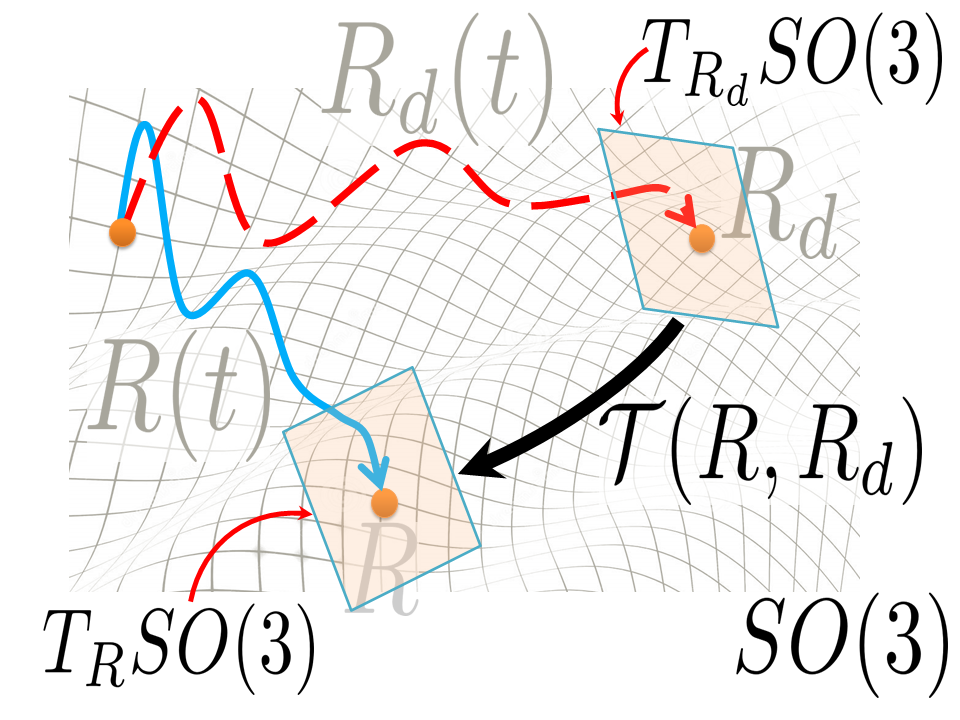
\includegraphics[width=.45\textwidth]{./StyleStuff/transport.png}}
	\caption{Transport map $ \mathcal{T}(q,r) $\label{fig:con.transport}}
\end{figure}		
%The tracking error $ \Psi_R $ and the transport map $ \mathcal{T}(q,r) $ allow the definition of error between velocity curves.

%The time derivative of the tracking error function is defined by the tracking error function $ \Psi_R $, the transport map $ \mathcal{T}(q,r)  $ and the velocity error curve $ \dot{e} $. 
% $ \dot{e} $ is a function of the transport map $ \mathcal{T}(q,r)  $. 
%Where 
The \textit{velocity error} $ \dot{e} $ is a vector field along $ R $ corresponding to the transport map.
% $ \mathcal{T}(q,r) $. 
It defines the velocity error between the curves $ R$ and $ R_d$, and is defined as
\begin{equation}\label{eq:con.dote}
\dot{e}=\dot{R}-\dot{R}_d(R_d^TR)
\end{equation}
This equation is rewritten to obtain the angular velocity tracking error, as follows
\begin{equation}\label{key}
\begin{aligned}
\dot{R}-\dot{R}_d(R_d^TR) &=R\hat{\Omega}-R_d\hat{\Omega}_d(R_d^TR) \\
&=R(\Omega)^\wedge-(RR^T)R_d\hat{\Omega}_dR_d^TR\\
&=R(\Omega)^\wedge-R(R^TR_d{\Omega}_d)^\wedge \\
&=R(\Omega-R^TR_d{\Omega}_d)^\wedge 
\end{aligned}
\end{equation}
The angular \textit{velocity tracking error} $ e_{\Omega} $ expressed in \BF  is defined as
\begin{align}\label{eq:con.eOmega}
e_\Omega&=\Omega- R^TR_d\Omega_d
\end{align}
Similar to the form of Equation \ref{eq:mod.R}, $ e_\Omega $ represents the angular velocity vector of the relative rotation matrix $ R_d^TR $, represented in \BF. Hence, it can be shown that the following equation holds
\begin{equation}\label{key}
\frac{d}{dt}(R^T_dR)=(R_d^TR)\hat{e}_\Omega
\end{equation}
%Having defined a measure 

***************************************\\
Bart: Wat is het verschil tussen de velocity error between curves R en Rd en angular velocity tracking error?\\
Nam: velocity error $ \dot{e} $ is velocity error tussen $ \dot{R} $ en $ \dot{R}_d $.  Angular velocity error $ e_\Omega $ is de angular velocity vector van $ R_d^TR $, dus verschil tussen $ \Omega $ en $ \Omega_d $.

***************************************\\

The values of the \a{qr} attitude tracking error $ e_R $ and the \a{qr} angular velocity tracking error $ e_\Omega $ 
are used later on to design control for the \a{qr} attitude.
%a controller can use this values to control

\subsubsection*{Load Attitude Error}
The load attitude dynamics evolve on $ \mathbb{S}^2 $ and its tangent space $ T\mathbb{S}^2 $, where the error of the load attitude is described in a similar approach.
The error between the load attitude $ q $ and the desired load attitude $ q_d $ is defined by the error function $ q_d^Tq $. Based on the error function, the tracking error function $ \Psi_q $ on $ \mathbb{S}^2 $ is chosen to be
\begin{equation}\label{eq:psiq}
\Psi_q=1-q_d^Tq
\end{equation}
The derivative of the tracking error function $ \Psi_q $ is given by 
\begin{equation}\label{key}
d_1\Psi_q(q,q_d)=\hat{q}^2q_d
\end{equation}
From this equation, the load attitude error function $ e_q $ is defined as follows
\begin{equation}\label{eq:con.eq}
e_q=\hat{q}^2q_d
\end{equation}
Again, a \textit{transport map} is used for a comparison between the tangent vectors on different tangent spaces.
Using the tracking error $ \Psi_q $ and the transport map $ \mathcal{T}_{\mathbb{S}^2} $, a closed-loop energy function evolving on $ \mathbb{S}^2 $ is derived \cite[11.3.2]{Bullo2005}. From this energy function, the load angular velocity error function is defined as
\begin{equation}\label{eq:con.edq}
e_{\dot{q}}=\dot{q}-(q_d\times\dot{q}_d)\times q
\end{equation}
The values of the load attitude tracking error $ e_q $ and the load angular velocity tracking error $ e_{\dot{q}}$ 
are used later on to design control for the load attitude.

\subsubsection*{Load Position Error}
The tracking errors for the load position and load velocity are defined as
\begin{align}\label{key}
e_x&=x-x_d\\
e_v&=v-v_d
\end{align}
where $ v_d=\dot{x}_d $. Furthermore, $ x_d(t) \in \mathbb{R}^3$ must be a smooth twice-differentiable load trajectory, such that functions are well defined. The values of the position error $ e_x$ and the velocity error $ e_v $ are used later on to design control for the load position.

\newpage
\section{Backstepping Control}\label{sec:con.back}
A backstepping approach will be used in this research for the control of the load trajectory tracking problem, and is commonly used \a{qr} control\cite{Mahony2012}. Backstepping control is a Lyapunov based control technique for the stabilization of nonlinear dynamical systems developed by \cite{Kanellakopoulos1991}. 
The method relies on a \textit{triangular structure} of the system in a certain set of coordinates. The system is split into subsystems in a cascaded structure and recursive techniques allow a systematically design of feedback control laws and corresponding Lyapunov functions.\\
The control structure is created by starting with a stable system as the most inner subsystem. 
By "stepping back" from this subsystem, a control loop can be added around it containing a control law that defines a change of coordinates, which allows control of a new state, while still stabilizing the inner structure. The control law is designed by using states as virtual control inputs, such that each loop computes a virtual command signal for the adjacent inner loop. This is repeated until the final external control is reached.\\
The backstepping approach determines how to stabilize the \a{qr} with the control inputs $ f $ and $ M $, while several controllers are able to track different states, see Figure \ref{fig:con.loop}. 
The inner controller determines what the required control inputs are, driven by $ R_c $.  
The next controller calculates how to drive the computed rotation matrix $ R_c $ based on $ q_c $, such that the \a{qr} is stabilized.
And the last controller determines which load attitude $ q_c $ is required, such that the desired load position $ x_{L,d} $ is tracked.
\begin{figure}[h!]
	\centering
	\makebox[\textwidth][c]{\includegraphics[trim={0 0 0 12cm},clip,width=.95\textwidth]{./StyleStuff/backstepQR3.png}}
	\caption{Nonlinear Geometric Control Loop of the QR-Load system \cite{Sreenath2013c}\label{fig:con.loop}}
\end{figure}	

% EXTRA LINK
%\url{https://www.slideshare.net/ieijjournal/feedback-linearization-and-backstepping-controllers-for-coupled-tanks}
%\url{http://www.control.lth.se/media/Education/EngineeringProgram/FRTN05/2013/lec09_2013eight.pdf}
%We want to design a state feedback u=u(x) that stabilizes
%\begin{equation}\label{key}
%\begin{aligned}
%\dot{x}_1&=f(x_1)+g(x_1)x_2\\
%\dot{x}_2&=u
%\end{aligned}
%\end{equation}
%Idea is to see system as a cascade connection. Design controller first for inner loop, then for the outer.
%
%Back-Stepping Lemma
%\textbf{Lemma}: Let $ z=\begin{pmatrix}x_1,\cdots,x_{k-1}\end{pmatrix}^T$ and 
%\begin{equation}\label{key}
%\begin{aligned}
%\dot{z}&=f(z)+g(z)x_k\\
%\dot{x}_k&=u
%\end{aligned}
%\end{equation}
%Assume $ \phi(0)=0 $, $ f(0)=0 $,
%\begin{equation}\label{key}
%\dot{z}=f(z)+g(z)\phi(z)
%\end{equation}
%stable, and $ V(z) $ a Lyapunov function (with $ \dot{V}\leq-W $). Then, 
%\begin{equation}\label{key}
%u=\frac{d\phi}{dz}\begin{pmatrix}
%f(z)+g(z)x_k
%\end{pmatrix}-\frac{dV}{dz}g(z)-(x_k-\phi(z))
%\end{equation}
%stabilizes $ x=0 $ with $ V(z)+(x_k-\phi(z))^2/2 $ begin a Lyapunov function.
%
%The backstepping approach determines how to stabilize the {\displaystyle \mathbf {x} } \mathbf {x}  subsystem using {\displaystyle z_{1}} z_{1}, and then proceeds with determining how to make the next state {\displaystyle z_{2}} z_{2} drive {\displaystyle z_{1}} z_{1} to the control required to stabilize {\displaystyle \mathbf {x} } \mathbf {x} . Hence, the process "steps backward" from {\displaystyle \mathbf {x} } \mathbf {x}  out of the strict-feedback form system until the ultimate control {\displaystyle u} u is designed.
%***************************************\\

Since the \a{qr} has only four actuators, it is not possible to control all \a{DOF}s of the \a{qr}-Load system simultaneously. The backstepping approach allows control of different flight modes in which a combination of \a{DOF}s are controlled. The flight modes and their functions are defined below in order, from the most inner loop to the most outer loop.
\begin{outline}
	\1 QR Attitude Controlled Mode 
	\2 Track a desired QR attitude $ R_d(t) $ or commanded signal $ R_c(t) $. Optional tracking of a desired heading direction $ b_{1_d}(t) $, the first column of $ R_d(t) $.
	\2 Calculate the control input $ M $ for the \a{qr}-Load system
	\1 Load Attitude Controlled Mode 
	\2 Track a desired load attitude $ q_d(t) $ or commanded signal $ q_c(t) $
	\2 Calculate a computed \a{qr} attitude $ R_c $ for the \a{qr} attitude controller
	\2 Calculate the control input $ f $ for the \a{qr}-Load system	
	\1 Load Position Controlled Mode
	\2 Track a desired load position $ x_{L,d}(t) $
	\2 Calculate a computed load attitude $ q_c $ for the load attitude controller
	\2 Calculate the control input $ f $ for the \a{qr}-Load system		
\end{outline}

***************************************\\
Bart: Dit wist ik niet. Waar komt heading direction vandaan. Is nergens anders gedefinieerd in je document\\
Nam: b1d is een extra state die nog getracked kan worden in deze controller, het is een kolom van $ R_d $, maar hoeft niet per se. Kan er voor zorgen dat de QR niet rondjes gaat draaien. Later wordt b1d, b1c en definieert hiermee Rc. Iets veranderd boven, duidelijk?

***************************************\\
where the subscript $d $ denotes a desired tracking reference, and the subscript $ c $ denotes a computed tracking reference, calculated by the controllers. 
%CHECK NODIG??
More detailed derivations of the equations in the following sections can be found in Section \ref{sec:app.error}.
%value that is calculated as a . The difference in this notation is whether the signal is a predefined desired signal, or a signal computed by a controller.
%The controller that is used in this research is shown in Figure \ref{fig:con.loop}. The lowest levels have the highest bandwidth and are in control of the rotor rotational speeds $ \omega_i $, the total force $ f $ and moments $ M $. The next level controls the load attitude $ q $, and the top level controls the load position $ x_L $. 

\subsection{Quadrotor Attitude Tracking}\label{sec:con.qratt}
The \a{qr} Attitude Controlled Mode is designed to control the \a{qr} attitude by tracking a smooth desired \a{qr} attitude $ R_d(t) $.  
Analysis of the error dynamics $ e_R $ and $ e_\Omega $ requires the calculation of their time derivatives.\\
Using Equations \ref{eq:con.eR} and \ref{eq:con.eOmega}, the derivative of the attitude tracking error $ e_R $ can be written as
\begin{equation}\label{key}
\dot{e}_R=\frac{1}{2}(R_d^TR\hat{e}_\Omega+\hat{e}_\Omega R^TR_d)^\vee
\end{equation}
The derivative of the angular velocity tracking error $ e_\Omega $, follows from Equations \ref{eq:mod.R}, \ref{eq:con.eOmega} and the fact that $ \hat{\Omega}_d\Omega_d =0$, such that
\begin{equation}\label{eq:con.deOmega}
\dot{e}_\Omega=\dot{\Omega}+\hat{\Omega}R^TR_d\Omega_d-R^TR_d\dot{\Omega}_d
%\dot{e}_\Omega=J^{-1}(-\Omega\times J\Omega + M)+\hat{\Omega}R^TR_d\Omega_d-R^TR_d\dot{\Omega}_d
\end{equation}
Recall from Equation \ref{eq:mod.R}, that the kinematics equation for the desired attitude can be written as
\begin{equation}\label{eq:con.dotRd}
\dot{R}_d=R_d\hat{\Omega}_d \text{ and } \hat{\Omega}_d=R_d^T\dot{R}_d
\end{equation}
From this follows that the desired angular acceleration $ \dot{\Omega}_d $ can then be defined as follows
\begin{equation}
\begin{aligned}
\dot{\hat{\Omega}}_d&=(\dot{R}_d^T\dot{R}_d)+(R_d^T\ddot{R}_d)\\
&=(R_d\hat{\Omega}_d)^T(R_d\hat{\Omega}_d)+(R_d^T\ddot{R}_d)\\
&=-\hat{\Omega}_d\hat{\Omega}_d+R_d^T\ddot{R}_d,\\
\dot{\Omega}_d&=(-\hat{\Omega}_d\hat{\Omega}_d+R_d^T\ddot{R}_d)^\vee \label{eq:con.dOmegad}
\end{aligned}
\end{equation}
By substituting Equation \ref{eq:mod.qratt} into Equation \ref{eq:con.deOmega}, the following is obtained
\begin{equation}\label{eq:con.dOmega}
\dot{e}_\Omega=J^{-1}(-\Omega\times J\Omega + M)+\hat{\Omega}R^TR_d\Omega_d-R^TR_d\dot{\Omega}_d
\end{equation}
From this, the control input $ M $ is defined \cite{Lee2010c}, and consists of a proportional term, a derivative term and a canceling term, as follows
\begin{equation}\label{eq:con.M}
M = -k_Re_R-k_\Omega e_\Omega+\Omega\times J\Omega-J(\hat{\Omega}R^TR_d\Omega_d-R^TR_d\dot{\Omega}_d)
\end{equation}
Rapid exponential convergence of the attitude error function and angular velocity error function can be achieved by adding
the parameter \lsymb{$ \epsilon $}{Tuning parameter to enable rapid exponential convergence of $ e_R, e_\Omega $} to
Equation \ref{eq:con.M}, where $ 0<\epsilon<1 $, as done in \cite{Sreenath2013c}
\begin{equation}\label{eq:con.Meps}
M = -\frac{1}{\epsilon^2}k_Re_R-\frac{1}{\epsilon}k_\Omega e_\Omega+\Omega\times J\Omega-J(\hat{\Omega}R^TR_d\Omega_d-R^TR_d\dot{\Omega}_d)
\end{equation}
Substituting Equation \ref{eq:con.Meps} into Equation \ref{eq:con.dOmega} results in
\begin{equation}\label{eq:con.JdeOmega}
\dot{e}_\Omega=J^{-1}(-\frac{1}{\epsilon^2}k_Re_R-\frac{1}{\epsilon}k_\Omega e_\Omega)
\end{equation} 
for any positive constants $ k_R, k_\Omega $.\\
% and where \lsymb{$ \epsilon $}{Tuning parameter to enable rapid exponential convergence of $ e_R, e_\Omega $} is the parameter to enable rapid exponential convergence of the attitude- and angular velocity error functions, such that $ 0<\epsilon<1 $ \cite{Sreenath2013c}
%such that Equation \ref{eq:con.deOmega} is reduced to
%\begin{equation}\label{eq:con.JdeOmega}
%J\dot{e}_\Omega=-k_Re_R-k_\Omega e_\Omega
%\end{equation}
%for any positive constants $ k_R, k_\Omega $.\\
Equation \ref{eq:mod.hattrace} is used to rewrite the time derivative of $ e_R $ as follows
 %rewrite the attitude velocity error $ \dot{e}_R $ as follows
 \begin{equation}\label{eq:con.deR}
 \begin{aligned}
 \dot{e}_R&=\frac{1}{2}(R_d^TR\hat{e}_\Omega+\hat{e}_\Omega R^TR_d)^\vee\\
 &=\frac{1}{2}(tr[R^TR_d]I-R^TR_d)e_\Omega \equiv C(R_d^TR)e_\Omega 
 \end{aligned}
 \end{equation}
where $ \parallel C(R_d^TR)\parallel_2\leq 1 $, such that $ \parallel\dot{e}_R\parallel\leq\parallel e_\Omega \parallel  $ for all $ R^T_dR\in SO(3) $, guaranteeing that $ \dot{e}_R $ will be bounded if $ e_\Omega $ is. 
Equations \ref{eq:con.JdeOmega} and \ref{eq:con.deR} are used in a stability analysis of the controller, and it is proven in \cite{Lee2010} 
that the zero equilibrium of the closed loop tracking error $ (e_R,e_\Omega)=(0,0) $ is exponentially stable, if the initial conditions satisfy
\begin{equation}\label{eq:dom1}
\Psi_R(R(0),R_d(0))<2
\end{equation}
\begin{equation}\label{eq:dom2}
\parallel e_\Omega(0)\parallel^2<\frac{2}{\lambda_M(J)}\frac{k_R}{\epsilon^2}(2-\Psi_R(R(0),R_d(0)))
\end{equation}
where \lsymb{$ \lambda_M(\cdot) $}{Maximum eigenvalue} denotes the maximum eigenvalue. \\
Furthermore, there exist constants $ \alpha_R,\beta_R>0 $ such that
\begin{equation}\label{eq:con.proofPsiR}
\Psi_R(R(t),R_d(t)) \leq min\left\lbrace 2,\alpha_Re^{-\beta_Rt}\right\rbrace 
\end{equation}
%T is defined by Equations . 
Equations \ref{eq:dom1} and \ref{eq:dom2} determine the domain of attraction, which is the region in which the trajectory of the system is able to converge to an asymptotically stable equilibrium point. 
The domain of attraction almost covers $ SO(3) $, this is referred to as almost-global exponential attractiveness.

Note that the tracking of the \a{qr} attitude does not require any specification of the thrust magnitude $ f $. During this flight mode, the translational motion can only be controlled partially, which makes this flight mode suitable for attitude maneuvers with short time periods.

\subsection{Load Attitude Tracking}\label{sec:con.loadatt}
%ADD Dependent of what values? 	How to choose parameters.
The Load Attitude Controlled Mode is designed to track a desired load attitude $ q_d $.
In order to influence the load dynamics, see Equation \ref{eq:mod.loadatt}, the load attitude controller calculates a computed \a{qr} attitude $ R_c $ for the \a{qr} attitude controller, such that
$ R_d $ is replaced by $ R_c $, where $ R_c $ is defined as
\begin{equation}\label{eq:con.R}
R_c = \begin{bmatrix}
b_{1c}; b_{3c}\times b_{1c};b_{3c}
\end{bmatrix}
\end{equation}
And $ \Omega_d $ is replaced by $ \Omega_c $, where $ \Omega_c $ is defined by
\begin{equation}\label{key}
\hat{\Omega}_c=R_c^T\dot{R}_c
\end{equation}
which will influence the \a{qr} attitude dynamics, see Equation \ref{eq:mod.qratt}.\\
The unit vector $ b_{1c} $ is the first column of $ R_c $ and is constructed by normalizing the projection of a desired heading angle $ b_{1d}\in \mathbb{S}^2 $ onto the plane normal to $ b_{3c} $, see Figure \ref{fig:con.b1c}. 
\begin{figure}[h!]
	\centering
	\makebox[\textwidth][c]{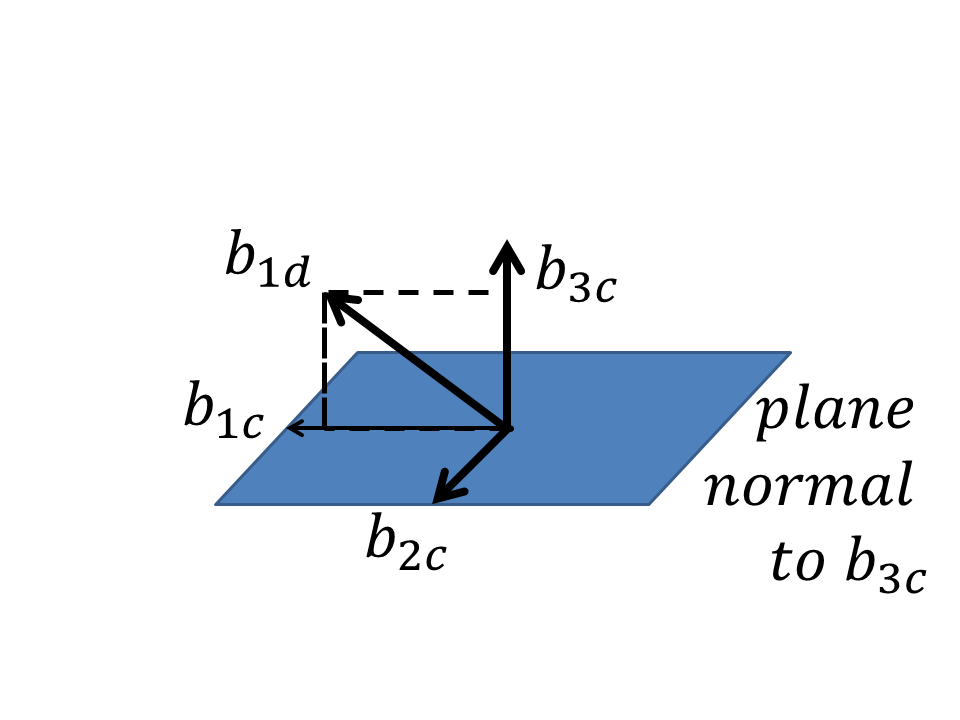
\includegraphics[trim={0 3cm 0 6cm},clip,width=.45\textwidth]{./StyleStuff/b1c.png}}
	\caption{Representation of $ R_c $\label{fig:con.b1c}}
\end{figure}	
Defining $ b_{1c}\in\mathbb{S}^2$ orthogonal to  $ b_{3c}$ guarantees that $ R_c \in SO(3) $ \cite{Lee2010c}.
This is defined as 
\begin{equation}\label{key}
b_{1c}=-\frac{1}{||b_{3c}\times b_{1d}||}(b_{3c}\times(b_{3c}\times b_{1d}))
\end{equation}
such that $ b_{1d} $ is chosen, not parallel to $ b_{3c} $. \\
$ b_{3c} \in \mathbb{S}^2 $ is the third column of $ R_c $ and is defined by a normalization of $ F $,
\begin{equation}\label{eq:con.b3c}
b_{3c}=\frac{F}{||F||}
\end{equation}
where $F $ is defined by a normal component $ F_n $, a proportional-derivative component $ F_{pd} $ and feedforward control force $ F_{ff}$
\begin{equation}\label{eq:con.F}
F=F_n-F_{pd}-F_{ff}
\end{equation}
% Control forces for a system  are derived . 
The inclusion of $ F_n $ ensures that $ b_{3c} $ is always well defined. $ F_n $ is defined as
\begin{equation}\label{eq:con.Fn}
F_n=-(q_d\cdot q)q
\end{equation}
The control forces $ F_{pd} $ and $ F_{ff} $ are defined for trajectory tracking in \cite[11.2.5]{Bullo2005} as follows
\begin{equation}\label{key}
\begin{aligned}
F_{pd}&=-k_P\hat{q}^2q_d-k_D(\dot{q}-(q_d\times\dot{q}_d)\times q)\\
&=-k_qe_q-k_\omega e_{\dot{q}}
\end{aligned}
\end{equation}
for positive constants $ k_q, k_\omega $.\\
\begin{equation}\label{key}
F_{ff}=m_QL\langle\!\langle q,q_d\times\dot{q}_d\rangle\!\rangle_{\mathbb{R}^3}(q\times \dot{q})+m_QL(q_d\times \ddot{q}_d)\times q
\end{equation}
	
This controller affects the control input $ f $, which is defined as
\begin{equation}\label{eq:con.fLoadatt}
f=F\cdot Re_3
\end{equation}
and the control input $ M $ will be defined as
\begin{equation}\label{eq:con.MLoadatt}
M = -\frac{1}{\epsilon^2}k_Re_R-\frac{1}{\epsilon}k_\Omega e_\Omega+\Omega\times J\Omega-J(\hat{\Omega}R^TR_c\Omega_c-R^TR_c\dot{\Omega}_c)
\end{equation} 

It is proven in \cite{Sreenath2013c} and \cite[Lemma 11.23]{Bullo2005} that the zero equilibrium of the closed loop tracking error $ (e_q,e_{\dot{q}},e_R,e_\Omega)=(0,0,0,0) $ is exponentially stable, if the initial conditions satisfy
\begin{equation}\label{eq:dom3}
\Psi_q(q(0),q_d(0))<2
\end{equation}
\begin{equation}\label{eq:dom4}
\parallel e_{\dot{q}}(0)\parallel^2<\frac{2}{m_QL}{k_R}(2-\Psi_q(q(0),q_d(0)))
\end{equation}

The domain of attraction is defined by Equations \ref{eq:dom1}, \ref{eq:dom2}, \ref{eq:dom3} and \ref{eq:dom4}. Equation \ref{eq:dom3} states that the initial load attitude error should be less than $ 180^\circ $, which means that the controller achieves almost-global exponential convergence for load attitude $ q $.
Furthermore, there exist constants $ \alpha_q,\beta_q>0 $ such that
\begin{equation}\label{eq:con.proofPsiq}
\Psi_q(q(t),q_d(t)) \leq min\left\lbrace 2,\alpha_qe^{-\beta_qt}\right\rbrace 
\end{equation}

\subsection{Load Position Tracking}\label{sec:con.loadpos}
The Load Position Controlled Mode is designed to track a desired load position $ x_{L,d} $. 
Analysis of the error dynamics $ e_x $ and $ e_v $ requires the calculation of their time derivatives.\\
The derivative of the load position error $ e_x $ is given by
\begin{equation}\label{eq:con.dex}
\dot{e}_x = e_v
\end{equation}
and from Equation \ref{eq:mod.loadpos} and given that $ \dot{e}_v=\ddot{x}_L-\ddot{x}_{L,d} $ follows
\begin{equation}\label{eq:con.dev}
(m_Q+m_L)\dot{e}_v=-(m_Q+m_L)(ge_3+\ddot{x}_{L,d})-m_QL(\dot{q}\cdot\dot{q})q+(q\cdot fRe_3)q
\end{equation}
Equations \ref{eq:con.dex} and \ref{eq:con.dex} are used in a stability analysis of the controller. 
The load position controller calculates a computed load attitude $ q_c$ for the load attitude controller. $ R_d $ and $ q_d $ are replaced by $ R_c $ and $ q_c $, respectively. 
In order to stabilize the error dynamics, it is proven in \cite{Sreenath2013c} that the required computed load attitude is defined as
\begin{equation}\label{eq:con.q}
q_c = - \frac{A}{||A||}
\end{equation}
where
\begin{equation}\label{key}
A = -k_xe_x-k_ve_v+(m_Q+m_L)(\ddot{x}_{L,d}+ge_3)+m_QL(\dot{q}\cdot\dot{q})q
\end{equation}
%with $ e_x=x_L-x_{L,d} $ and $ e_v=\dot{x}_L-\dot{x}_{L,d} $.
Furthermore, Equation \ref{eq:con.Fn} is redefined as
\begin{equation}\label{key}
F_n=(A\cdot q)q
\end{equation}
which is substituted in Equation \ref{eq:con.F}, resulting in a new control input $ f $. 

This controller ensures that the zero equilibrium of the closed loop tracking error $ (e_x,e_v,e_q,e_{\dot{q}},e_R,e_\Omega)=(0,0,0,0,0,0) $ is exponentially attractive, if the initial conditions satisfy
\begin{equation}\label{eq:dom5}
\Psi_q(q(0),q_c(0))<\psi_1<1
\end{equation}
\begin{equation}
\parallel e_{x}(0)\parallel^2<e_{x_{max}}
\end{equation}
where $ e_{x_{max}} $ and $ \psi_1 $ are fixed design depended constants. 

The domain of attraction is defined by Equations \ref{eq:dom1}, \ref{eq:dom2}, \ref{eq:dom5} and the following equation
\begin{equation}
\parallel e_{\dot{q}}(0)\parallel^2<\frac{2}{m_QL}{k_q}(\psi_1-\Psi_q(q(0),q_d(0)))
\end{equation}

%\section{Stability Analysis}\label{sec:con.sta}
%
%Normally Lyapunov Analysis is 
%
%
%Lyapunov Analysis on SO3 x R3 and S2 x R3
%
%
%
%%In addition, the LaSalle invariance result and related Lyapunov results apply to closed-loop vector fields defined on these manifolds. 
%
%However, since the manifolds $ SO(3) $ and $ \mathbb{S}^2 $ are compact, the radial unboundedness assumption cannot be satisfied; consequently, global asymptotic stability cannot follow from a Lyapunov analysis on Euclidean spaces [40], and therefore must be analyzed in alternative ways [19]–[23].\cite[p.43]{Chaturvedi2011}
%
%[40]:
%[19]:
%[20]:
%[21]:
%[22]:
%[23]:
%
%
%\cite{Chaturvedi2011} summarizes global results on attitude control and stabilization for a rigid body using continuous time- invariant feedback. The analysis uses methods of geometric mechanics based on the geometry of the special orthogonal group $ SO(3) $ and the two-sphere $ \mathbb{S}^2 $.
%
%%ADD 
%%Justify choice of parameters. Up to what level can we push the system? Where can we find more info about domain of attractions.
%%How to choose parameters and how to select gains for errors


\section*{Summary}
In this chapter, control design based on Nonlinear Geometric Control is discussed.
%It is pointed out that 
%The main difference 
What is particular in this control technique, is the fact that error functions are defined on non-Euclidean manifolds, similar to the manifolds that describe the configuration space of the system.
Since these manifolds are locally Euclidean, local stability properties of a closed-loop equilibrium solution can be determined by using standard Lyapunov methods. 
Based on these error functions, controllers are designed in a backstepping approach, enabling both load position tracking and stabilization of the system.
Using the geometric properties of the system allows the design of globally defined controllers that ensure almost-global convergence of the \a{qr} attitude and load attitude.
In order to test the control performance of a load position tracking objective, experiments are defined in the next chapter. 

% CHECK Chaturvadi?
%Stability analysis is different from a Lyapunov analysis on Euclidean spaces.









\chapter{Experiments and Results}\label{ch:results}
%ADD intro: in this section etc
In Section \ref{sec:set.setup} the experimental setup is explained. The chosen model- and controller parameters are presented.

The experiments that are used are explained and discussed in Section \ref{sec:set.exp}, of which the results are presented and discussed in Section \ref{sec:set.exp}.

A conclusion is made based on the obtained results in Section \ref{set:set.res}.

\section{Setup}\label{sec:set.setup}
\paragraph{Model parameters}
%ADD chosen model parameters 
The simulations are developed using Matlab and Simulink, using the following system parameters.
\begin{equation}\label{key}
\begin{aligned}
J&=\\
m_Q&=\\
\nonumber
\end{aligned}
\quad
\begin{aligned}
d&=\\
c_{\tau f}&=\\
\nonumber
\end{aligned}
\quad
\begin{aligned}
m_L&=\\
l_L&=\\
\nonumber
\end{aligned}
\end{equation}

\paragraph{LQR Control}
\a{lqr} control is based on small angle assumption. Therefore, a traditional modeling method may represent the rotation matrix with a local coordinate system, for example with a Euler Angle parameterization. An \a{lqr} control design is based on a linearized model of the system. The control design is shown in Figure \ref{fig:set.lqr} and the derivation of the model can be found in Section \ref{app:lqr}.
\begin{figure}[h!]
	\centering
	\makebox[\textwidth][c]{\includegraphics[width=.45\textwidth]{./StyleStuff/dcsc.png}}
	\caption{LQR control design\label{fig:set.lqr}}
\end{figure}		

%ADD chosen parameters LQR
The tuning parameters of the \a{lqr} controller a chosen as follows
\begin{equation}\label{key}
A=\begin{bmatrix}
content...
\end{bmatrix}
\end{equation}
\begin{equation}\label{key}
B=\begin{bmatrix}
content...
\end{bmatrix}
\end{equation}
\begin{equation}\label{key}
C=\begin{bmatrix}
content...
\end{bmatrix}
\end{equation}

where the state $ \mathbf{x} $ and input $ u $ are defined as 
\begin{align}\label{eq:state}
\textbf{x}&=\begin{bmatrix}
\textbf{q}\\
\mathbf{\dot{q}}
\end{bmatrix}\\
\mathbf{q}&=\begin{bmatrix}
x&y&z&\phi&\theta&\psi&\theta_L&\psi_L
\end{bmatrix}^T\\
\mathbf{\dot{q}}&=\begin{bmatrix}
\dot{x}&\dot{y}&\dot{z}&\dot{\phi}&\dot{\theta}&\dot{\psi}&\dot{\theta}_L&\dot{\psi}_L
\end{bmatrix}^T\\
u&=\begin{bmatrix}
f&M_\phi&M_\theta&M_\psi
\end{bmatrix}^T
\end{align}

\paragraph{Geometric Control}
%ADD chosen parameters GC
The controller gains in Equations \ref{eq:con.M},\ref{eq:con.R},\ref{eq:con.q} are chosen to be
\begin{equation}\label{key}
\begin{aligned}
k_R&=\\
k_\Omega&=\\
\end{aligned}
\quad
\begin{aligned}
k_q&=\\
k_\omega&=\\
\end{aligned}
\quad
\begin{aligned}
k_x&=\\
k_v&=
\nonumber
\end{aligned}
\end{equation}


\subsection{Command Filtering}
%ADD Why is Command Filtering needed? 
Implementation of the backstepping approach also increases the order of the states. Thus, a consequence of backstepping control is that inner control loops become a function of the commanded signals and their higher derivatives, generated by an outer loop.
Instead of analytic differentiation of these terms, which can be tedious and require high computational costs, these values can be obtained with the use of a Command Filter, which is explained in more detail in \cite{Farrell2008}.

Basically, the command signal is pre-filtered by a low pass filter 

with the following state space representation
%CHECK waar dit ook alweer vandaan kwam. Reference in Djapic/Farell -> 3e order voor bacterieen ofzo
\begin{align}\label{key}
\dot{x}_1 &= x_2\\ %dxc
\dot{x}_2 &= x_3\\ %ddxc
\dot{x}_3 &= -(2\zeta \omega_{n2}+\omega_{n1})x_3-(2\zeta\omega_{n1}\omega_{n2}+\omega_{n2}^2)x_2-(\omega_{n1}\omega_{n2}^2)(x_1-x_c^o)
\end{align}
where $ x_1 = x_c$, $ x_2 = \dot{x}_c$ and $ x_3 = \ddot{x}_c$. 

The transfer function of the original commanded input signal $ X_c^o $ and the filtered output $ X_c $ has the form
\begin{equation}\label{key}
\frac{X_c(s)}{X_c^o(s)}=H(s)=\frac{\omega_{n1}}{s+\omega_{n1}}\cdot\frac{\omega_{n2}^2}{s^2+2\zeta\omega_{n2}s+\omega_{n2}^2}
\end{equation}
Where $ \zeta $ is the damping ratio and $ \omega_n $ the undamped natural frequency. See Figure \ref{fig:set.CF} and \ref{fig:app.CF}.

This command filter is implemented to compute $ \dot{R}_c, \ddot{R}_c,\dot{q}_c, \ddot{q}_c $.
%\begin{equation}\label{key}
%
%\end{equation}

%CHECK
%Examples from \cite{Farrell2008} and \cite{Djapic2008}. 

***************************************\\
%ADD Pro Con Command filter
Easy implementation. Less computational effort.

Less accurate, because filters high frequency signals.

***************************************\\

The load attitude controller generates a commanded QR attitude $ R_c $ and its derivative $ \dot{R}_c $. In the same fashion, the load position controller generates a commanded load attitude $ q_c $ and its derivative $ \dot{q}_c $. 

The controllers are functions of these commanded signals and their derivatives. Instead of analytic differentiation of these signals, they are obtained by integration by applying a third order low pass filter to the original signals $ R_c^o $ and $ q_c^o $. 
The state space implementation of this third order filter is \cite{Djapic2008}


\begin{figure}[h!]
	\centering
	\makebox[\textwidth][c]{\includegraphics[width=.45\textwidth]{./StyleStuff/dcsc.png}}
	\caption{Representation of the command filter\label{fig:set.CF}}
\end{figure}		

\begin{align}\label{eq:CF}
\frac{x_c}{x_c^o}&=\frac{\omega_{n1}}{s+\omega_{n1}}\cdot\frac{\omega_{n2}^2}{s^2+2\zeta\omega_{n2}s+\omega_{n2}^2}\\
\Rightarrow x_c^{'''}&=-(2\zeta\omega_{n2}+\omega_{n1})x_c^{''}-(2\zeta\omega_{n1}\omega_{n2}+\omega_{n2}^2)x_c^{'}-(\omega_{n1}\omega_{n2} ^2)(x_c-x_c^o)
\end{align}

\section{Experiments}\label{sec:set.exp}

\a{lqr} is an optimal control strategy and will be used to compare its result to a Nonlinear Geometric Controller.

$ x_d(t) $ is required to be smooth for the Geometric Control. Trajectories are generated by hand, however it is possible to compute these with trajectory generating algorithms too.

\subsection{Performance Criteria}
Performance  that can be evaluated for different cases can be specified by the following
\begin{outline}
	\1 Step Response
	\2 Settling time (if swing minimization is important)
	\2 Rising time (important if time critical)
	\2 Overshoot (if max swing is critical)
	\2 Steady state error / swing of load (if accuracy is important)
	\2 Max load angle
	
	\1 Disturbance Rejection
	
	\1 Trajectory tracking
	\2 Can we minimize time, while minimizing position error (All Cases)
	\2 Minimum position error (All Cases)
	\2 Maximum amplitude/frequency of wave with respect to stability (Case B)
	
	\1 Computational Effort (?)
\end{outline}

%ADD 
%Explain cases, why interesting and what can be expected?\\

\subsection{Case A}
%ADD 
%Explain cases, why interesting and what can be expected?\\

From point A to point B

%ADD xdes
%ADD inputs f M
%ADD QR attitude
%ADD 

\subsection{Case B}
%ADD 
%Explain cases, why interesting and what can be expected?\\


\subsection{Case C}
%ADD 
%Explain cases, why interesting and what can be expected?\\

%CHECK nog nodig?
%\begin{figure}[h!]
%	\centering
%	\makebox[\textwidth][c]{\includegraphics[width=.2\paperwidth]{./StyleStuff/dcsc.png}}
%	\caption{Cases of which the performance could be evaluated \label{fig:routes}}
%\end{figure}

\section{Results}\label{set:set.res}
\subsection{Case A}


\subsection{Case B}


\subsection{Case C}


\section{Conclusion}\label{set:set.con}
%CHECK 
%What can we learn and conclude from different performance comparisons

%What is its value of nonlinear control compared to linear control

%No restrictions on rotor direction. is it possible to turn 2 ways?

%Could it be interesting for a real-time on-board controller
%Considering the computational power of an on-board processor is limited
%computational effort vs what?

\chapter{Conclusions and Future Work}\label{ch:conclusion}
%ADD in this section etc

\section{Summary and Conclusions}
This report starts by introducing the subject.
The aim is described and the motivation for this research is given.

After the main introduction, the concepts of Geometric Mechanics are introduced. 
Instead of the trivial Euclidean spaces defined by Cartesian coordinates, the configuration space of the model is described on nonlinear manifolds.
This approach is used to obtain a model through the tools of Differential Geometry. 

Based on the geometric model, a nonlinear geometric control design is discussed.  
A backstepping approach, allows different \a{DOF}s of the under-actuated system to be controlled in a cascaded structure. 
The geometric control is based on 
 are functions
of error functions defined on nonlinear manifolds.
by Differential Geometry. 

Next, the experiment is defined. The nonlinear controller is used to track desired load trajectories in different situations. The nonlinear performance is compared to an \a{lqr} control 
Testing the nonlinear Geometric Controller
To compare with a common linear controller, \a{lqr} control is used to compare
Results are,

The conclusions that can be extracted from the experiments is that 

\section{Recommendations for Future Work}\label{ch:future}
% DONT make it look like literature survey. Based on details, show what I have learned. What could be interesting next. What is missing for the next steps.

\subsection{Investigate Implementation}
%Lack of time: no implementation possible. 
%In order to realize this, one needs to investigate the subjects

\paragraph{Digital Control} The concept of Geometric Control is shown under the assumption of continuous-time control. 
However, an analysis must be done in the discrete-time domain for the implementation of a real-time application. This must verify whether it is feasible to run the controller on an on-board processor on a \a{qr}. The control performance could be limited by the bandwidth of either the discretized control system or the wireless communication.
It must be investigated whether the control system is still able to deal with the fast dynamics that are required for aggressive maneuvering. 
Continuous-time Euler-Lagrange equations could be found by minimizing the action integral, which is a function of the Lagrangian. In a similar procedure the discrete-time Euler-Lagrange can be obtained, by minimizing te summation of a discrete Lagrangian, which is demonstrated in \cite{Lee2008}. 
%ADD reference Lee, digital geometric control. computed
%Computational Geometric Mechanics and Control\\
%\cite{Lee2008}
%Computation algorithms must be developed which preserve the geometric properties of a mechanical system.\\

\paragraph{Model identification and validation}
In this thesis the model parameters are either obtained from examples in literature or arbitrarily chosen. In practice, identification and validation of the \a{qr} model and rotor dynamics is required.
The mathematical model requires inclusion of the masses, inertia matrix and lengths of the \a{qr}, as well as the drag and thrust constants of the rotors, that are very unlikely to be identical.

As a theoretical extension the influence of model mismatches could be simulated.

\paragraph{Robustness}
The control in this thesis assumes perfect state feedback. In practice the controller depends on visual feedback or data obtained from an on-board inertial measurement unit. Unlike in simulations, this data will contain noise, uncertainties and possibly drift. 
Based on a nonlinear geometric approach for a \a{qr} without load, \cite{Goodarzi2013a} includes uncertainties in the translational dynamics and rotational dynamics to prove the robustness against unstructured uncertainties. This work could be extended to a \a{qr}-Load system to investigate the effects of non-perfect. 

%\subsection{Modeling Constraints}

%CHECK is dit uberhaupt nodig
%There are several techniques to handle input saturation, the most popular ones are anti-windup techniques. Back-calculation is such a method for PID to activate the integrator, is this possible for NL control?

%CHECK
%State estimation 

%CHECK
%Model Uncertainties
%\cite{Goodarzi2013a} includes uncertainties in the translational dynamics and rotational dynamics. Out of the scope, might be interesting.

\subsection{Minimum Snap Trajectory Generation}
The trajectories described in Section \ref{sec:set.traj} were arbitrarily generated by hand to test the performance of the controller in different situations. 
Whenever more complex trajectories are desired, or when an optimal trajectory is required, this approach is no longer efficient and too complex to solve by hand.
A recommended extension to this thesis is the automatic generation of a trajectory. 
This can be done as presented by \cite{Mellinger2011} and applied in \cite{Tang2014,Tang2015}, where a \acs{qp} problem is solved by minimizing the second derivative of the acceleration (snap),  guaranteeing a smooth optimal trajectory. The \a{qp} allows inclusion of input constraints and other requirements. 
It is proven that the system is \textit{differential flat}, meaning that all states and inputs can be expressed in terms of only four states and their derivatives. This property is used to transform the high-dimensional optimization problem into a four-dimensional problem.

\subsection{Hybrid System}
This thesis is only focused on the subsystem where the tension in the cable is non-zero. A possible extension is to apply hybrid control, such that the controller is able to switch between two subsystem models whenever the cable tension switches between zero and non-zero. 
A trajectory generation method that accounts for the switching dynamics of the hybrid system is presented in \cite{Tang2014}. 
%\include{future_work}

%LATEX TEST
%\part{TEST PARTS}
%\chapter{Trajectory Generation}\label{ch:trajectory}

***************************************\\
Trajectory is first generated by hand. A simple trajectory that will not push the system to its limits yet\\
Next, trajectory can be generated by solving a \a{QP} via minimum snap generation.

***************************************\\

Trajectory Generation by minimizing Snap Trajectory. QP.\\

\section{Minimum Snap Trajectory Generation}


\section{Conclusion}


%
% First Part
    \part{First Part}

    \chapter{First Real Chapter}

%    This is real chapter for \ac{DUT}, ok? I will explain everything about \gsymb{$\gamma$}{Path Angle}. Next, everything
%    will be explained about the transfer function \lsymb{$H(s)$}{Transfer function}. Also, subscripts and can
    superscripts can be put in the nomenclature \index{nomenclature} list. 
%    \supers{max}{Maximum} 
%    \subs{min}{Minimum} 
    Other things can also
    be added to the nomenclature list of \ac{DUT} 
%    \others{[kts]}{Knots} \others{$^{\circ}$, [deg]}{Degrees}

        \section{First section}

        This is the section. Referring to equations, figures and tables can easily be done by the commands \verb"\eqnref{}",
        \verb"\figref{}" and \verb"\tabref{}".
        \begin{equation}\label{eq:First}
              H(s) = \frac{1}{s+2}
        \end{equation}
        You see? Refer to equations like this \eqnref{eq:First}.
            \subsection{The first subsection}

                \subsubsection[Subsection Short Title]{The first sub-subsection with a very very very long title, but in the table of contents one can only see the short title}

                Nice, ain't it?\index{Nice}

                    \paragraph{A paragraph.}
    \part{Second part}

    \chapter{Second part chapter}
   \begin{figure}
    \caption{this is a very long line to test if the table of
    figures will wrap the line or will continue to go over the
    border  of the page}
    \end{figure}

    \chapter{TEMP second part chapter this is a very long line to test if the table of
    figures will wrap the line or will continue to go over the
    border  of the page}

New chapter gives a full acronym \ac{TU}.

\begin{eqnarray}
% \nonumber to remove numbering (before each equation)
  1 &=& 2\\
  x &=& 5 \\
  y &=& \theta
\end{eqnarray}

    \chapter{Second second part chapter}
    \section{Section}

    This is a test for nomenclature \lsymb{$A(s)$}{Answer function}\\
    \lsymb{$a_f$, $b_f$, $c_f$ and $d_f$}{The variables I am trying to group}\\
    \lsymb{$a_b$}{another variable}\\
\section{Main equations}

\begin{equation}
a=\frac{N}{A}
\end{equation}%

\nomenclature{$a$}{The number of angels per unit area}%
\nomenclature{$N$}{The number of angels per needle point}%
\nomenclature{$A$}{The area of the needle point}%

The equation $\sigma = m a$%
\nomenclature{$\sigma$}{The total mass of angels per unit area}%
\nomenclature{$m$}{The mass of one angel}
follows easily.


	
%============================= Appendices=========================================
\appendix
\chapter{Appendix}

\section{Derivation of Equations of motion}
\subsection{Load Dynamics}\label{sec:app.loaddyn}
%PROOF prop.3 Sreenath2013a. Also Sreenath2013b?
%DEFINE e_3 / R / f 

Let \lsymb{$ x_{CM} $}{Position CM of \a{qr}-Load system} denote the position of the center of mass of the combined Quadrotor-Load system, expressed in \IF. Which can be found by
\begin{align}\label{eq:CM}
\begin{split}
m_Q(x_Q-x_{CM})+m_L(x_L-x_{CM})&=0\\
(m_Q+m_L)x_{CM}&=m_Qx_Q+m_Lx_L
\end{split}
\end{align}
Applying Newton's laws of motion to (\ref{eq:CM}) and inserting (\ref{eq:mod.xQ2xL}) gives the 
\begin{align}\label{key}
\begin{split}
(m_Q+m_L)\ddot{x}_{CM}&=fRe_3 - (m_Q+m_L)ge_3\\
%&=fRe_3 - (m_Q+m_L)ge_3\\
%(m_Q+m_L)\ddot{x}_{CM}&=m_Q\ddot{x}_Q + m_L\ddot{x}_L\\
%\\
%m_Q\ddot{x}_Q+m_L\ddot{x}_L&=fRe_3 - (m_Q+m_L)ge_3\\
%m_Q(\ddot{x}_L-L\ddot{q})+m_L\ddot{x}_L&=fRe_3 - (m_Q+m_L)ge_3\\
(m_Q+m_L)(\ddot{x}_L+ge_3)&= fRe_3+m_QL\ddot{q}
\end{split}
\end{align}

%ADD derivation of ddq (TANG2014)
Here comes the derivation of $ \ddot{q} $, obtained by geometric mechanics.

\section{LQR controller}\label{app:lqr}

\subsection{Modeling}
%From Newton's laws follows
%\begin{align}
%x_Q&=fRe_3-m_Qge_3-Tq\\
%x_L&=-m_Lge_3+Tq
%\end{align}
%
%$ x_Q $ and $ x_L $ are related by
%\begin{equation}\label{key}
%x_L = x_Q+Lq
%\end{equation}

%CHECK is dit nodig?
% From Lagrangian equations of motion, 
%
%\begin{equation}\label{eq:app.QRpos}
%\begin{aligned}
%%ADD Not done yet
%\ddot{x}&=\\
%\ddot{y}&=\\
%\ddot{z}&=
%\end{aligned}
%\end{equation}
%
%\begin{equation}\label{eq:app.QRatt}
%\begin{aligned}
%%ADD Not done yet
%\ddot{\phi}&=\\
%\ddot{\theta}&=\\
%\ddot{\psi}&=
%\end{aligned}
%\end{equation}
%
%\begin{equation}\label{eq:app.Latt}
%\begin{aligned}
%%ADD Not done yet
%\ddot{\phi}_L&=\\
%\ddot{\theta}_L&=
%\end{aligned}
%\end{equation}
%The second order system of ODEs can be transformed 
The linearized model is written into a first order ODE of the form
\begin{align}\label{eq:app.ss}
\mathbf{\dot{x} }&=A\mathbf{x}+Bu\\
y&=C\mathbf{x}+Du
\end{align}
with the following state- and input vectors
\begin{equation}\label{key}
\begin{aligned}
%\textbf{x}&=\begin{bmatrix}
%\textbf{q}\\
%\mathbf{\dot{q}}
%\end{bmatrix}\\
%\mathbf{q}&=\begin{bmatrix}
%x&y&z&\phi&\theta&\psi&\phi_L&\theta_L
%\end{bmatrix}^T\\
%\mathbf{\dot{q}}&=\begin{bmatrix}
%\dot{x}&\dot{y}&\dot{z}&\dot{\phi}&\dot{\theta}&\dot{\psi}&\dot{\phi}_L&\dot{\theta}_L
%\end{bmatrix}^T\\
\mathbf{x}&=\begin{bmatrix}
x&y&z&\phi&\theta&\psi&\phi_L&\theta_L&\dot{x}&\dot{y}&\dot{z}&\dot{\phi}&\dot{\theta}&\dot{\psi}&\dot{\phi}_L&\dot{\theta}_L
\end{bmatrix}^T\\
u&=\begin{bmatrix}
f&M_\phi&M_\theta&M_\psi
\end{bmatrix}^T
\end{aligned}
\end{equation}

The model is linearized about the hovering flight mode. All translational and rotational velocities are zero during hover. The positional states and the yaw angle do not affect the dynamics, and are set equal to zero. A thrust input $ u_1=g(mQ+mL) $ is required to maintain hover, and all other control inputs are set equal to zero. 
The states and inputs in the equations of motion are substituted by an initial condition and a perturbation
\begin{equation}\label{key}
\mathbf{\dot{x}}\rightarrow\mathbf{\dot{x}}_0+\delta\mathbf{\dot{x}}, \quad \mathbf{{x}}\rightarrow\mathbf{{x}}_0+\delta\mathbf{{x}}, \quad u\rightarrow u_0+\delta u
\end{equation}
\begin{equation}\label{key}
\begin{aligned}
\mathbf{x}(0) &= \mathbf{0}\\
u(0)&=\begin{bmatrix}
g(m_Q+m_L) &0 &0& 0
\end{bmatrix}^T
\end{aligned}
\end{equation}
The linearized equations of motion are rearranged into Equation \ref{eq:app.2ode} and substituted in Equation \ref{eq:app.ss}.
\begin{equation}\label{eq:app.2ode}
\begin{bmatrix}
content...
\end{bmatrix}
\begin{bmatrix}
		\delta \ddot{x} \\\delta\ddot{y}\\\delta\ddot{z}\\\delta\ddot{\phi}\\\delta\ddot{\theta}\\\delta\ddot{\psi}\\\delta\ddot{\phi}_L\\\delta\ddot{\theta}_L 
		\end{bmatrix}+
\begin{bmatrix}
content...
\end{bmatrix}
\begin{bmatrix}
		\delta {x} \\\delta{y}\\\delta{z}\\\delta{\phi}\\\delta{\theta}\\\delta{\psi}\\\delta{\phi}_L\\\delta{\theta}_L 
\end{bmatrix}
=
\begin{bmatrix}
content...
\end{bmatrix}
\begin{bmatrix}
\delta u_1\\\delta u_2\\\delta u_3\\\delta u_4
\end{bmatrix}
\end{equation}

%ADD LQRA
\begin{lstlisting}
LQRA =

\end{lstlisting}
%ADD LQRB
\begin{lstlisting}
LQRB =

\end{lstlisting}
The tuning parameters of the \a{lqr} controller a chosen as follows
%TEST different values LQR
\begin{equation}\label{key}
\begin{aligned}
Q &= diag\begin{pmatrix}
10 &10 &100,& 1& 1& 1, &1& 1,& 1& 1 &1,& 1& 1& 1,& 1& 1
\end{pmatrix}\\
R &= diag\begin{pmatrix}
0.044, &1.56,& 1.56, &1.56
\end{pmatrix}
\end{aligned}
\end{equation}
\texttt{Matlab} command \texttt{lqr(LQRA,LQRB,Q,R)} generates the following gain matrix $ K $
%ADD K
\begin{lstlisting}
K =

\end{lstlisting}




%CHECK useful? Praveen EOM
%	    \begin{equation}
%	    ax = 
%	    \begin{bmatrix}
%	    f(ms_{\phi_q}s_{\psi_q}+ m_Ls_{\phi_q}s_{\psi_q} + mc_{\phi_q}c_{\psi_q}s_{\theta_q} + m_Lc_{\phi_q}c_{\psi_q}s_{\theta_q}- m_Lc_{\phi_q}c_{\psi_q}c_{\theta}^2s_{\theta_q} + m_Lc_{\phi}^2c_{\phi_q}c_{\psi_q}c_{\theta}^2s_{\theta_q} - m_Lc_{\theta}^2s_{\phi_q}s_{\psi_q}+ m_Lc_{\phi}^2c_{\theta}^2s_{\phi_q}s_{\psi_q}  + m_Lc_{\psi_q}c_{\theta}s_{\phi}s_{\phi_q}s_{\theta} + m_Lc_{\phi}c_{\phi_q}c_{\theta_q}c_{\theta}^2s_{\phi} - m_Lc_{\phi_q}c_{\theta}s_{\phi}s_{\psi_q}s_{\theta_q}s_{\theta})
%	    
%	    
%	    (   + Lmm_Lv_\theta^2c_{\theta}s_{\phi} + Lmm_Lv_\phi^2c_{\theta}^3s_{\phi} )/(m(m + m_L))\\
%	    \\
%	    (Lmm_Lv_\theta^2s_{\theta} - fm_Lc_{\psi_q}c_{\theta}^2s_{\phi_q} - fmc_{\psi_q}s_{\phi_q} + fmc_{\phi_q}s_{\psi_q}s_{\theta_q} + fm_Lc_{\phi_q}c_{\theta}^2s_{\psi_q}s_{\theta_q} + Lmm_Lv_\phi^2c_{\theta}^2s_{\theta} + fm_Lc_{\phi}c_{\phi_q}c_{\theta_q}c_{\theta}s_{\theta} - fm_Lc_{\theta}s_{\phi}s_{\phi_q}s_{\psi_q}s_{\theta} - fm_Lc_{\phi_q}c_{\psi_q}c_{\theta}s_{\phi}s_{\theta_q}s_{\theta})/(m(m + m_L))\\
%	    \\
%	    -(gm^2 + gmm_L - fmc_{\phi_q}c_{\theta_q} - fm_Lc_{\phi_q}c_{\theta_q} + Lmm_Lv_\theta^2c_{\phi}c_{\theta} + fm_Lc_{\phi}^2c_{\phi_q}c_{\theta_q}c_{\theta}^2 + Lmm_Lv_\phi^2c_{\phi}c_{\theta}^3 + fm_Lc_{\phi}c_{\psi_q}c_{\theta}s_{\phi_q}s_{\theta} - fm_Lc_{\phi}c_{\theta}^2s_{\phi}s_{\phi_q}s_{\psi_q} - fm_Lc_{\phi}c_{\phi_q}c_{\theta}s_{\psi_q}s_{\theta_q}s_{\theta} - fm_Lc_{\phi}c_{\phi_q}c_{\psi_q}c_{\theta}^2s_{\phi}s_{\theta_q})/(m(m + m_L))\\
%	    \\
%	    (- Lmc_{\theta}s_{\theta}v_\phi^2 + fc_{\psi_q}c_{\theta}s_{\phi_q} - fc_{\phi}c_{\phi_q}c_{\theta_q}s_{\theta} - fc_{\phi_q}c_{\theta}s_{\psi_q}s_{\theta_q} + fs_{\phi}s_{\phi_q}s_{\psi_q}s_{\theta} + fc_{\phi_q}c_{\psi_q}s_{\phi}s_{\theta_q}s_{\theta})/(Lm)\\
%	    \\
%	    -(fc_{\phi_q}c_{\theta_q}s_{\phi} + fc_{\phi}s_{\phi_q}s_{\psi_q} - 2Lmv_\phi v_{\theta}s_{\theta} + fc_{\phi}c_{\phi_q}c_{\psi_q}s_{\theta_q})/(Lmc_{\theta})
%	    \end{bmatrix}
%	    \end{equation}	    
%	    
%	    ***************************************\\	

\section{Classical Modeling}\label{sec:mod.clas}
This section describes the derivation of the model by using classical modeling techniques.

When assuming small angle maneuvers, \textit{Euler-angles} can be used to locally parameterize the orientation of the body-fixed reference coordinate frame with respect to the inertial reference coordinate frame. Simple linear controllers are often based on a linearized dynamical model, applying this small angles assumption. 

\begin{figure}[h!]
	\centering
	\makebox[.65\textwidth][c]{\subfloat[][Quadrotor model representation \label{fig:app.model}]{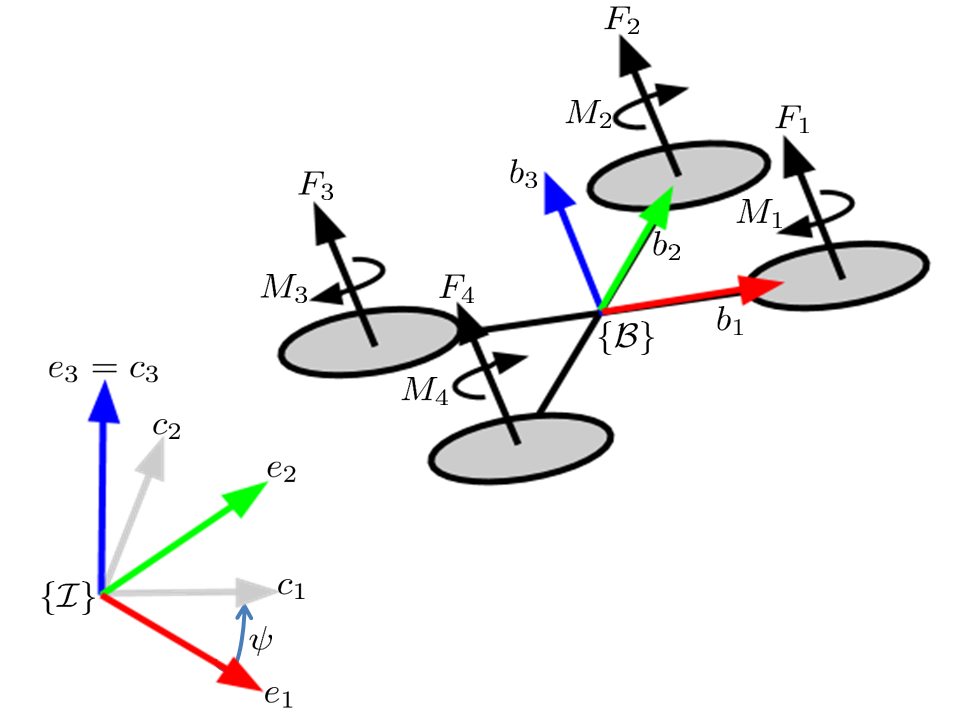
\includegraphics[width=.5\textwidth]{./StyleStuff/qrmodel.png}}}
	\makebox[.34\textwidth][c]{\subfloat[][Load angles  \label{fig:app.angles}]{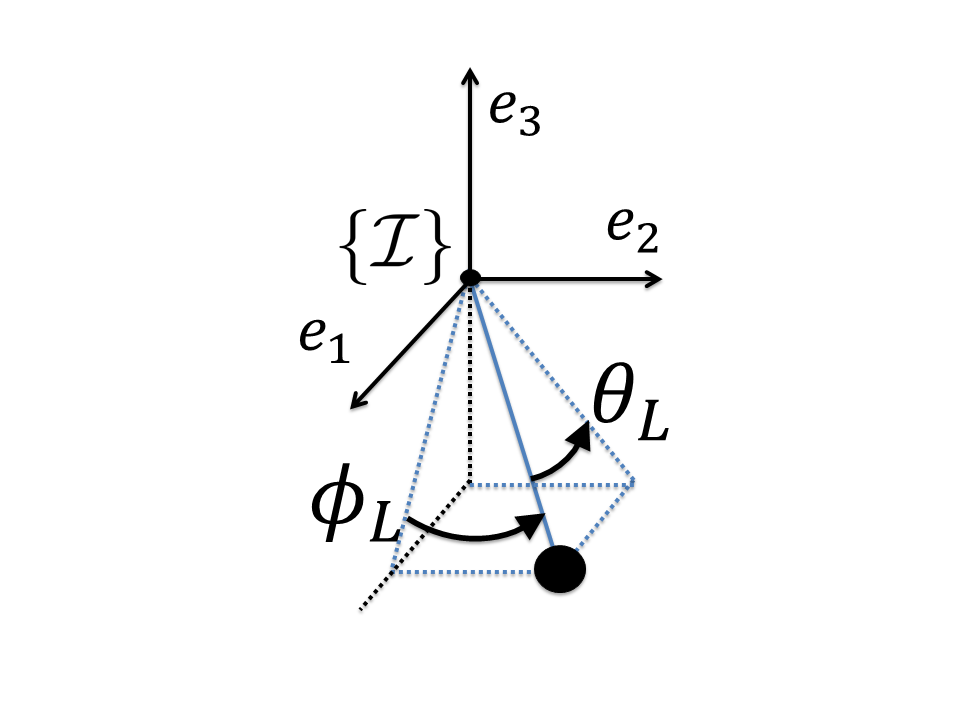
\includegraphics[width=.5\textwidth]{./StyleStuff/angles.png}}}
	\caption{Model representation\label{fig:}}
\end{figure}		

The following equations of motion follow from Newton's law.
\begin{equation}\label{eq:newton}
\begin{aligned}
\dot{x}_Q &= v_Q\\
m_Q\dot{v}_Q &=fRe_3-m_Qge_3-Tq\\
\dot{x}_L &= v_L\\
m_L\dot{v}_L &=-m_Lge_3+Tq
\end{aligned}
\end{equation}
where $ x_Q = x_L-Lq $. $ T $ is the cable tension, defined by $ T=|f| q $, where $ |f| = m_L\dot{v}_L $ is the magnitude of the force.
%which gives the following equation, derived in Section \ref{sec.app:loaddyn},
%\begin{equation}\label{key}
%%CHECK whether equation is correct
%(m_Q+m_L)(\dot{v}_L+ge_3)=fRe_3-m_QL\ddot{q}
%\end{equation}

Because Euler-Angles are used, a function is required that maps a vector of the Z-X-Y Euler angles to its rotation matrix $ R\in SO(3) $, which is denoted as \cite{Mahony2012}
\begin{equation}\label{key}
R_{ZXY}({\phi},{\theta},{\psi})=\begin{bmatrix}
c_{\psi}c_{\theta}-s_{\phi}s_{\psi}s_{\theta}&-c_{\phi}s_{\psi}&c_{\psi}s_{\theta}+c_{\theta}s_{\phi}s_{\psi}\\
c_{\theta}s_{\psi}+c_{\psi}s_{\phi}s_{\theta}&c_{\phi}c_{\psi}&s_{\psi}s_{\theta}-c_{\psi}c_{\theta}s_{\phi}\\
-c_{\phi}s_{\theta}&s_{\phi}&c_{\phi}c_{\theta}
\end{bmatrix}
\end{equation}
The Z-X-Y Euler angles rotate \BF, as can be seen in Figure \ref{fig:app.model}. The first rotation by yaw angle $ \psi $ is around the z-axis of \IF. Next is the rotation by roll angle $ \phi $, and the last rotation is by pitch angle $ \theta $.
%\begin{figure}[h!]
%	\centering
%	\makebox[\textwidth][c]{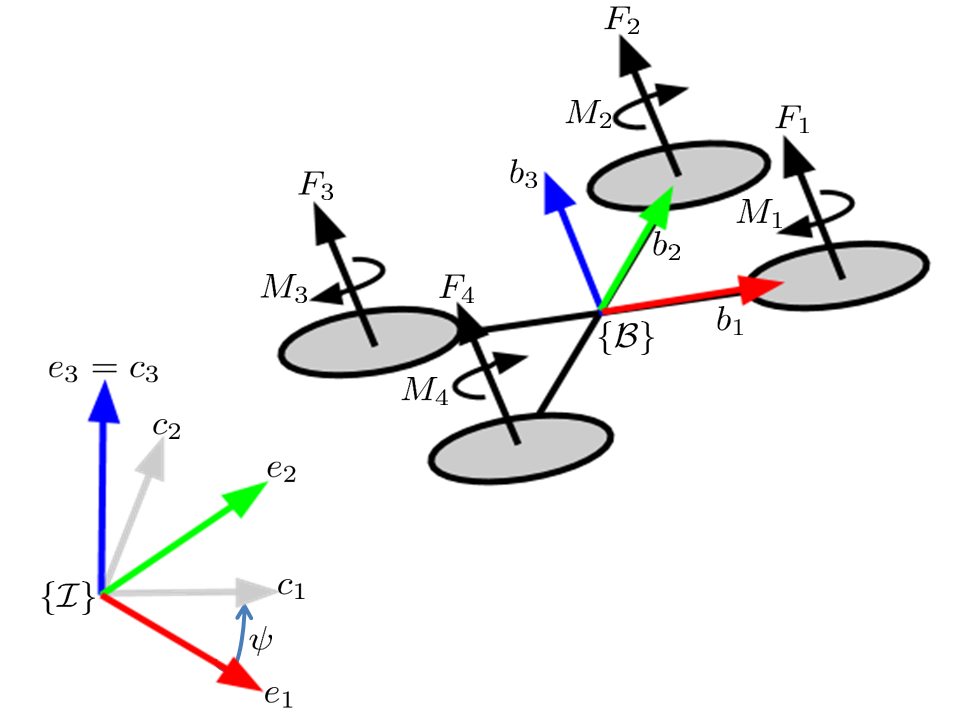
\includegraphics[width=.45\textwidth]{./StyleStuff/qrmodel.png}}
%	\caption{Quadrotor-Load model representation\label{fig:mod.modelQRtrad}}
%\end{figure}

The unit vector $ q $ from the \a{qr} to the load is represented in \BF. Define $ \phi_L $ as the rotation of the load around the z-axis, measured from $ \vec{b}_1 $, and $ \theta_L $ is the angle between the cable and the z-axis of \BF, see Figure \ref{fig:app.angles}.
The Cartesian coordinates can be retrieved through
\begin{equation}\label{eq:app.xL2xQ}
x_L = x_Q+qL
\end{equation}
where
\begin{equation}\label{eq:app.q}
q=
\begin{bmatrix}
s_{\theta_L}c_{\phi_L}\\
s_{\theta_L}s_{\phi_L}\\
-c_{\theta_L}
\end{bmatrix}
\end{equation}
%\begin{figure}[h!]
%	\centering
%	\makebox[\textwidth][c]{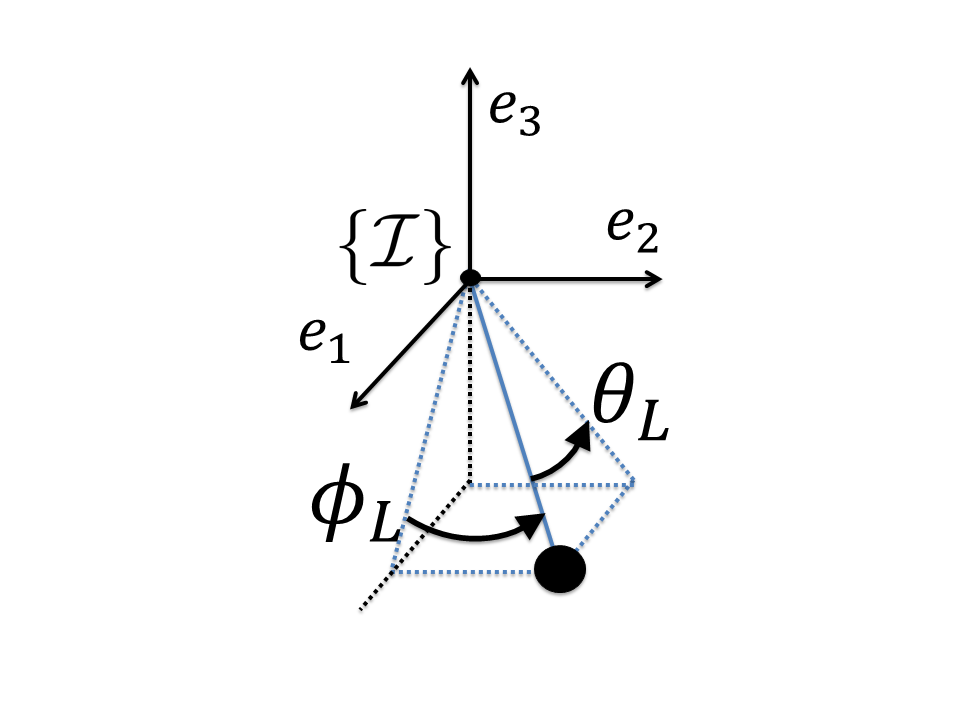
\includegraphics[width=.45\textwidth]{./StyleStuff/angles.png}}
%	\caption{Load angles \label{fig:app.angles}}
%\end{figure}	

%\begin{figure}[h!]
%	\centering
%	\makebox[\textwidth][c]{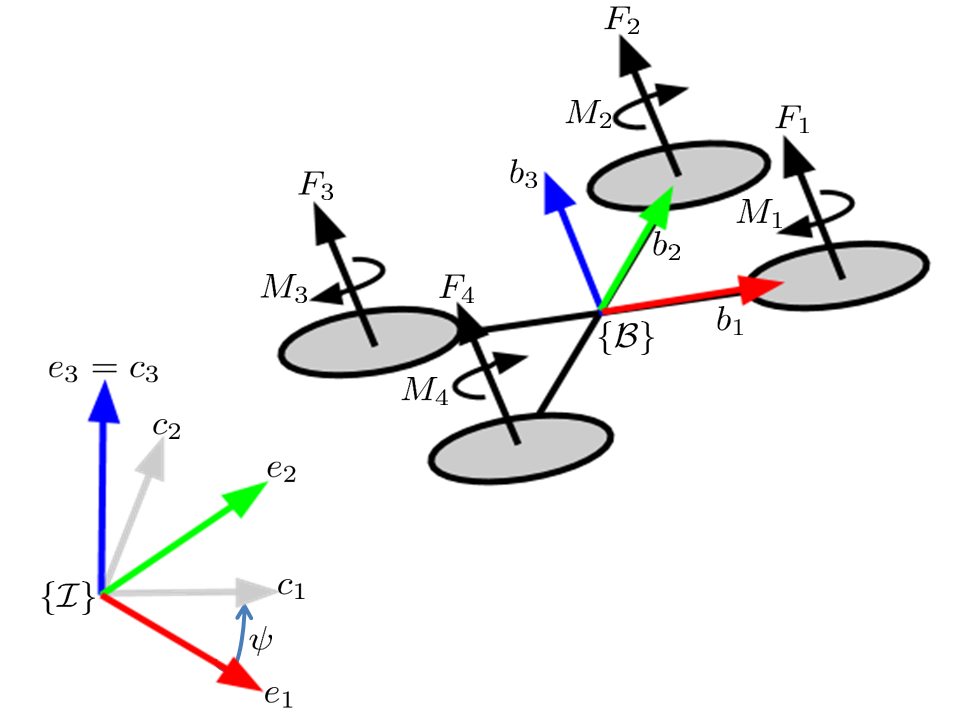
\includegraphics[width=.5\paperwidth]{./StyleStuff/qrmodel.png}}
%	\caption{Quadrotor model representation\label{fig:mod.model}}
%\end{figure}	



%\begin{equation}\label{eq:q}
%		q=-R_{\psi_L}R_{\theta_L}e_3=\begin{bmatrix}
%		s_{\theta_L}c_{\psi_L}\\s_{\theta_L}s_{\psi_L}\\-c_{\theta_L}
%		\end{bmatrix}
%\begin{align}
%q=\begin{bmatrix}
%s_{\theta_L}c_{\phi_L}\\
%s_{\theta_L}s_{\phi_L}\\
%c_{\theta_L}
%\end{bmatrix}
%\dot{q}&=\begin{bmatrix}
%s_{\theta_L}c_{\psi_L}\\
%s_{\theta_L}s_{\psi_L}\\
%c_{\theta_L}
%\end{bmatrix}\\
%\end{align}
%\end{equation}  
Differentiating Equation \ref{eq:app.xL2xQ} and \ref{eq:app.q} gives
\begin{equation}\label{key}
\begin{aligned}
\ddot{x}_L&=\ddot{x}_Q+\ddot{q}L\\
\ddot{q}&=\begin{bmatrix}
\ddot{\theta}_Lc_{\theta_L}c_{\phi_L}-\ddot{\phi}_Ls_{\theta_L}s_{\phi_L}-\dot{\phi}_L^2s_{\theta_L}c_{\phi_L}-\dot{\theta}_L^2s_{\theta_L}c_{\phi_L}-2\dot{\theta}_L\dot{\phi}_Lc_{\theta_L}s_{\phi_L}\\
\ddot{\theta}_Lc_{\theta_L}s_{\phi_L}+\ddot{\phi}_Ls_{\theta_L}c_{\phi_L}-\dot{\phi}_L^2s_{\theta_L}s_{\phi_L}-\dot{\theta}_L^2s_{\theta_L}s_{\phi_L}+2\dot{\theta}_L\dot{\phi}_Lc_{\theta_L}c_{\phi_L}\\
\ddot{\theta}_Ls_{\theta_L}+\dot{\theta}_L^2 c_{\theta_L}\\
\end{bmatrix}
\end{aligned}
\end{equation}

\begin{equation}\label{key}
\begin{aligned}
\ddot{x}_Q&=\frac{1}{m_Q}(f(c_{\psi}s_{\theta}+c_{\theta}s_{\phi}s_{\psi})-Ts_{\theta_L}c_{\psi_L})\\
\ddot{y}_Q&=\frac{1}{m_Q}(f(s_{\psi}s_{\theta}-c_{\psi}c_{\theta}s_{\phi})-Ts_{\theta_L}s_{\psi_L})\\
\ddot{z}_Q&=\frac{1}{m_Q}(f(c_{\phi}c_{\theta})-Tc_{\theta_L})-g\\
\end{aligned}
\end{equation}

%\begin{align}\label{key}
%%CHECK wat is hier de bedoeling van? Checken in Garcia of literatuur?
%\ddot{\psi}&=\tilde{\tau}_{\psi}\\
%\ddot{\theta}&=\tilde{\tau}_{\theta}\\
%\ddot{\phi} &=\tilde{\tau}_{\phi}
%\end{align}

\section{Figures}
\begin{figure}[h!]
	\centering
	\makebox[\textwidth][c]{\includegraphics[width=.45\textwidth]{./StyleStuff/dcsc.png}}
	\caption{Simulink Command Filter\label{fig:app.CF}}
\end{figure}		

\section{\texttt{MATLAB} code}
\subsection{A \matlab Listing}

\lstset{language=matlab}
\lstinputlisting{test.m}

%    \subsection{An appendix subsection with C++ Listing}
%
%    \lstset{language=C++}
%    \lstinputlisting{test.c}    

%    \chapter{Appendix: Figures}
%
%    \section{Test section (again?)}
%
%    Ok, all is well.


%============================= Back matter =========================================
\backmatter
	% Bibliography
	\bibliographystyle{ieeetr}
	\bibliography{library}
	
	%CHECK all entries for uniformity 	
	
	\printbib{library}
	
	% Index
	\printindex

	% Nomenclature
	\printnomenclature



\nonumchap{Acronyms}

\begin{acronym}[\hspace{0.8in}] % 0.8in is also used by the nomenclature
%	\acro{3mE}[3{m}E]{Mechanical, Maritime and Materials Engineering}%
%	\acro{DCSC}{Delft Center for Systems and Control}%
%	\acro{TU}[TU D{elft}]{Delft University of Technology}%

%	\acro{cmp}[CMP]{Cooperative Manipulation Problem}
%	\acro{atp}[ATP]{Aerial Towing Problem}

%	\acro{uav}[UAV]{Unmanned Aerial Vehicles}
%	
%	\acro{lti}[LTI]{Linear Time Invariant}
%	\acro{ltvmpc}[LTV MPC]{Linear Time Variant MPC}
%	\acro{mpc}[MPC]{Model Predictive Control}
%	\acro{mipc}[MIPC]{Mixed-Integer Predictive Control}	
%	\acro{nmpc}[NMPC]{Nonlinear Model Predictive Control}
%	\acro{mld-mpc}[MLD-MPC]{Mixed Logical Dynamical - Model Predictive Control}
%	\acro{lq}[LQ]{Linear Quadratic}

%
%	\acro{mld}[MLD]{Mixed Logical Dynamical}
%	\acro{pwa}[PWA]{Piecewise Affine}
%
%	\acro{aladin}[ALADIN]{Alternating Direction Inexact Newton method}
%	\acro{hysdel}[HYSDEL]{HYbrid Systems DEscription Language}	
%	\acro{dha}[DHA]{Discrete Hybrid Automata}
%	
%	\acro{lp}[LP]{Linear Programming}
%	\acro{dp}[DP]{Dynamic Programming}	
%	\acro{nlp}[NLP]{Nonlinear Program}

%	\acro{qcp}[QCP]{Quadratic Constrained Programming}	
%	\acro{qcqp}[QCQP]{Quadratically Constrained Quadratic Program}
%	
%	\acro{sqp}[SQP]{Sequential Quadratic Programming}
%	\acro{ip}[IP]{Interior Point}
%	
%	\acro{mip}[MIP]{Mixed Integer Programming}
%	\acro{milp}[MILP]{Mixed Integer Linear Programming}
%	\acro{miqp}[MIQP]{Mixed Integer Quadratic Programming}
%	\acro{miqcp}[MIQCP]{Mixed-integer Quadratically Constrained Programming}
%
%	
%
%	
%	\acro{ocp}[OCP]{Optimal Control Problem}
%	\acro{dae}[DAE]{Differential-Algebraic Equation}
%	
%	\acro{pd}[PD]{Proportional-Derivative}
%	\acro{pid}[PID]{Proportional-Integral-Derivative}
%	
%	\acro{rls}[RLS]{Recursive Least Squares}

	\acro{qr}[QR]{Quadrotor}
	\acro{uav}[UAV]{Unmanned Aerial Vehicle}

	\acro{com}[CoM]{Center of Mass}
	\acro{DOF}{Degree of Freedom}
	
	\acro{pid}[PID controller]{Proportional-Integral-Derivative Controller}
	\acro{mpc}[MPC]{Model Predictive Control}
	\acro{nmpc}[Nonlinear MPC]{Nonlinear Model Predictive Control}
	\acro{lqr}[LQR]{Linear Quadratic Regulator}
	
	\acro{qp}[QP]{Quadratic Programming}


\end{acronym}
	% Acronyms
%    \nonumchap{Acronyms}    
%    \begin{acronym}[XXXXX]% Note: replace XXXXX by the longest acronym
%                          %       in your list.
%        \acro{DUT}{Delft University of Technology}%
%    \end{acronym}%

\end{document}
